%--------------------------------
\section{Border Detection Experiments}
\label{cap6_result_experm_2}

The second set of experiments aimed to evaluate the method performance  in edge detection, a more complex and precise task than region segmentation.
BSDS500 was chosen due its small size, relative simplicity and its wide use in the literature, which makes it suitable for comparison to the literature.

BSDS500 consists in a set of 500 images with size of $480 \times 320$ pixels\footnote{~For boundary detection, images contains a extra pixel ($481 \times 321$ or $321 \times 481$)}.
The set is explicit subdivided into training, validation and test, containing 200, 100 and 200 images, respectively.
Ground truths are manually annotated by five different subjects on average. 
It contains ground truth for region segmentation and border detection \cite{amfm_pami2011}.

%{\color{blue}
%To visualize the data set and understand better the problem, Figure \ref{fig:bsds_colormap} was developed.
Unlike KITTI, BSDS data set does not contain pixels of interest (a.k.a. edges) distributed in a specific position of the image, making training difficult.
Also, the number non-edge pixels are considerably bigger than edge pixels \cite{ReExtraction:Wen201884}, becoming necessary to use methods that handles unbalanced classes, as discussed in the Section \ref{cap5_balanc_classes}.
%}

% \begin{figure}%[h!]
%   \centering
%   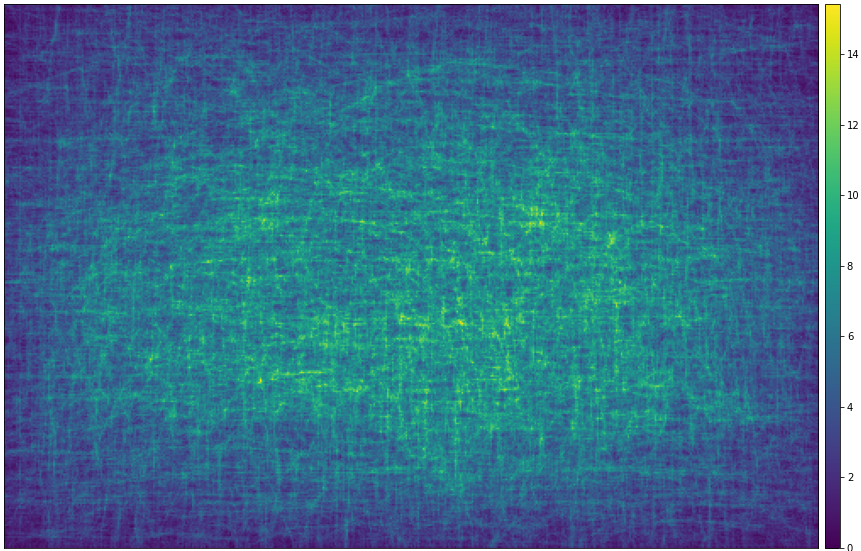
\includegraphics[width=1\columnwidth]{../imagens/visualiz_dados/bsds_colormap.png}
%   \caption{BSDS500 combined ground truth colormap.}
%   \label{fig:bsds_colormap}
% \end{figure}

BSDS500's test set is evaluated using BSDS500 Benchmark, provided by the authors \cite{amfm_pami2011}.
In our experiments, training and validation sets were merged into one group, in order to increase generalization.
The test set was only used to evaluate the performance of our results.

To increase training performance, it was used some data augmentation techniques, as salt and pepper noise, log and gamma contrast, JPEG compression, dropout, affine and perspective transformations, crop, pad, among others.
Rotation, flipping, mirroring and zoom (with factors of 0.5, 1.0 and 1.5) were combined with the techniques previously described.
All procedures resulted in 11400 images (38 samples per image).%\footnote{Code to generate these images are publicly available at \url{https://github.com/falreis/alo-seg-edge}}.
%The network was trained using 9690 images and validate on 1710 samples.
%Rotation procedure used the reflection technique to avoid cutting, empty regions or image size changing.

As previous experiments, the ground truth was separated into two binary classes, corresponding to the background and the edges.
However, after training, the system was changed to maintain classes, but to generate results based on confidence, in the range of 0 to 1, and no longer in binary form.
This method allows the identification of soft borders, as will be explained in the Section \ref{ssec:groundtruth_analysis}.%, and the definition of a border threshold, as \citeonline{Cumulative:Song20181847} paper.

Of all the experiments carried out, only a few important ones were detailed in this next subsections.
The analysis of experiments are summarized in Section \ref{cap6_discussion}.
%Other network architectures and test variations are available in Appendix \ref{apend:a}.

%--------------------------------
\subsection{Ground truth analysis}
\label{ssec:groundtruth_analysis}

As briefly reported previously, BSDS500's ground truths are manually annotated by five different subjects on average \cite{amfm_pami2011}.
Due multiples ground truths, some experiments were conducted to define how to combine them, in order to help the network to learn properly.
To do that, we developed and studied 3 different methods to combine them.

The first ground truth representation, named \textbf{ALL}, added all ground truths and divided them by the maximum of ground truths' overlaps in each image.
Ground truths borders were represented in a interval of 0 to 1, where the \textit{1-value} represents borders annotated in all ground truths, while the \textit{0-value} represents background in every annotation.
Values in between, correspond to soft borders, annotations marked in one or more ground truths but not in all them.
This representation is shown in Figure \ref{sfig:cap6_bsds_100075_all}.

\begin{figure*}%[h!]
  \centering
  \subfloat[\label{sfig:cap6_bsds_100075_orig_all}]{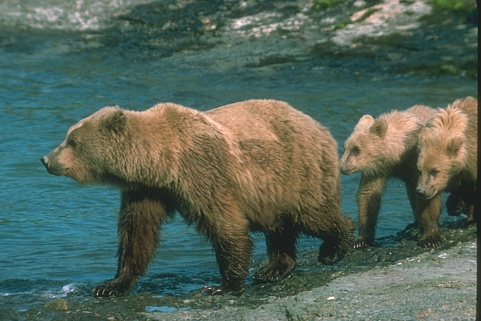
\includegraphics[width=0.24\textwidth]{../imagens/ilustracoes/cap6_bsds_100075.jpg}}
  \hfill
  \subfloat[\label{sfig:cap6_bsds_100075_all}]{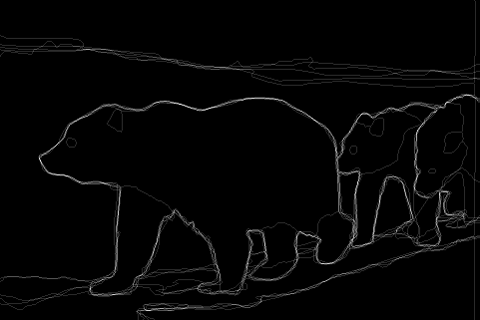
\includegraphics[width=0.24\textwidth]{../imagens/ilustracoes/cap6_bsds_100075_all.png}}
  \hfill
  \subfloat[\label{sfig:cap6_bsds_100075_upper}]{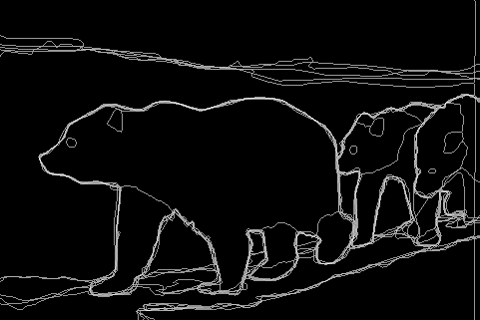
\includegraphics[width=0.24\textwidth]{../imagens/ilustracoes/cap6_bsds_100075_upper.png}}
  \hfill
  \subfloat[\label{sfig:cap6_bsds_100075_morf}]{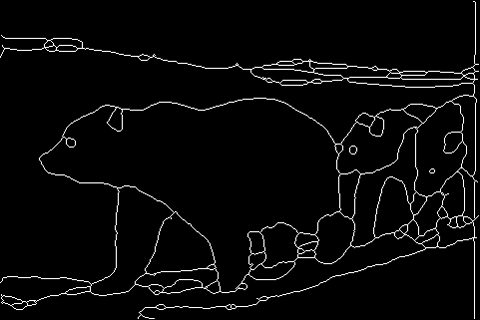
\includegraphics[width=0.24\textwidth]{../imagens/ilustracoes/cap6_bsds_100075_morf.png}}
  \caption{(a) BSDS500 image and its ground truth, using (b) ALL, (c) UPPER and (d) MORPH representations.}
  \label{fig:cap6_bsds_all}
\end{figure*}

This method had two major problems:

\begin{enumerate}
    \item As the number of ground truths for an image increases, some borders has really small values, almost close to the background value;
    \item Some borders are really close to others, but they do not overlap. So, the ground truth shows two different boundaries, which can make training difficult.
\end{enumerate}

One possible solution to fix the first problem is to limit boundaries to the interval of 0.5 to 1.0.
Background pixels are defined with value zero.
Once this method limited border in the upper range of values, it was named \textbf{UPPER}.
This ground truth representation method is available in Figure \ref{sfig:cap6_bsds_100075_upper}.

% \begin{figure}
%   \centering
%   \subfloat[\label{sfig:cap6_bsds_100075_orig_upper}]{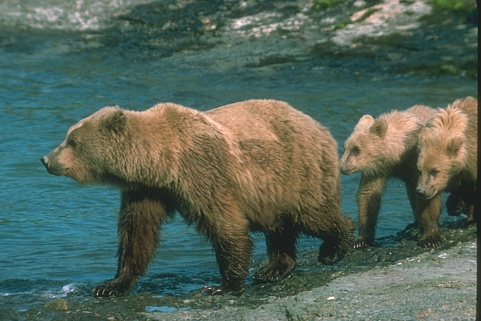
\includegraphics[width=0.48\textwidth]{../imagens/ilustracoes/cap6_bsds_100075.jpg}}
%   \hfill
%   \subfloat[\label{sfig:cap6_bsds_100075_upper}]{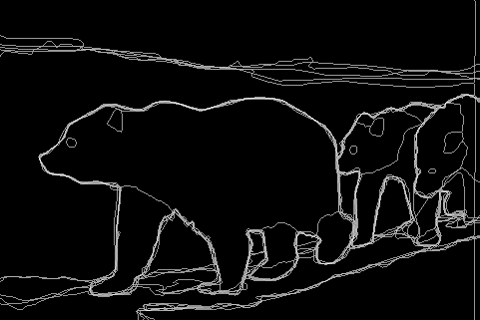
\includegraphics[width=0.48\textwidth]{../imagens/ilustracoes/cap6_bsds_100075_upper.png}}
%   \label{fig:cap6_bsds_upper}
%   \caption{(a) BSDS500 image and (b) its ground truth, using UPPER representation.}
% \end{figure}

Although benefits of the first approach, the second problem is not solved by them.
To settle it, an morphological set of operations were proposed to join close borders.
The chosen method corresponds to the dilatation of the boundaries using a kernel of $3 \times 3$, followed by a morphological thinning.
Dilation helps to join borders, but produced some shadows, that are removed by morphological thinning.

However, once morphological thinning is a binary operation, this method removes difference of values between borders, transforming soft borders into "hard borders", with values equal 1. 
The visual result of the morphological operations, named \textbf{MORPH}, is available in Figure \ref{sfig:cap6_bsds_100075_morf}.

% \begin{figure}
%   \centering
%   \subfloat[\label{sfig:cap6_bsds_100075_orig_morf}]{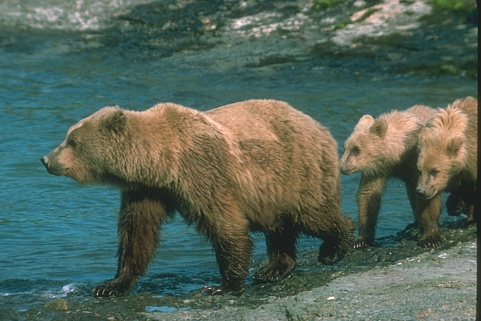
\includegraphics[width=0.48\textwidth]{../imagens/ilustracoes/cap6_bsds_100075.jpg}}
%   \hfill
%   \subfloat[\label{sfig:cap6_bsds_100075_morf}]{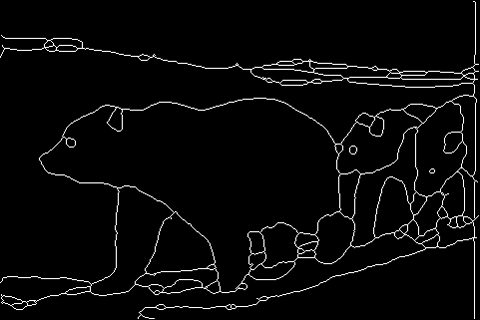
\includegraphics[width=0.48\textwidth]{../imagens/ilustracoes/cap6_bsds_100075_morf.png}}
%   \label{fig:cap6_bsds_morf}
%   \caption{(a) BSDS500 image and (b) its ground truth, using MORPH representation.}
% \end{figure}

Some initial experiments were performed to evaluate the three approaches.
It was observed that training the network using only ALL ground truth resulted into poor performance, due difficult of generalization.
The best generalization for early stage training was produced using MORPH ground truths.
However, ALL and UPPER ones, applied after a some MORPH training, produced better visual results.

%--------------------------------
\subsection{Protocol for experiments}
\label{ssec:framework_experiments}

%This section will describe the protocol developed for training our networks. 
As described in Section \ref{ssec:groundtruth_analysis}, the usage of ground truth \textit{MORPH} in the early stages of training achieved the best generalization.
After it, the usage of \textit{ALL} and \textit{UPPER} ground truths improves achieved results.
For this, we developed the following protocol, with the following phases:

\begin{enumerate}
    \item Train only deconvolutional layers with MORPH ground truth;
    \item Train the whole network with MORPH ground truth;
    \item Train the whole network using ALL or UPPER ground truths;
\end{enumerate}

The first step starts with pre-trained VGG16 model.
The results produced by first training phase, in terms of loss value, will be used by the following step.
Likewise, the second step produces the weights for third training phase.
At the end, the weights produced in the last phase are used to evaluate the network performance.

The following parameters set as standard in our experiments with BSDS500, unless otherwise specified:
\begin{itemize}
    \item Learning method: SGD
    \item Activation: ReLU
    \item Learning rate: $1 \times 10^{-6}$ (first phase) and $1 \times 10^{-7}$ (others)
    \item Decay: $1 \times 10^{-10}$ (first phase) and $1 \times 10^{-11}$ (others)
    \item Batch size: 8 images
    \item Merging method: ALO
    \item Loss: Focal Loss ($\gamma$=2.0; $\alpha$=0.25)\footnote{~Parameters recomended by \cite{Lin:2017} paper.}
    \item Initial weights: VGG-16
    \item Training samples: 9690 images 
    \item Validation samples: 1710 images
    \item Image size: $384 \times 288$
\end{itemize}

In addition to the parameters listed previously, it was decided to use some functions to automatically reduce the learning rate and finish the training procedure after a number of epochs without any improvements. 
Learning rate (LR) is reduced by factor of 0.3 ($LR \times 0.3$), after 10 epochs, if the loss does not decrease, in absolute value, at least 0.5 units\footnote{~This technique is also called as Reduce Learning Rate on Plateau.}.

After loss decreasing, the code waits for 5 epochs (\textit{cooldown}) and the procedure repeats until the learning rate achieves $1 \times 10^{-9}$, when it stops decreasing.
Concomitantly with learning rate reduction, the early stopping procedure finishes training when the absolute value does not decrease at least 0.5 units after 50 epochs.
If early stopping is not reached, the code will be completed after 1000 training epochs.

%--------------------------------
\subsection{Experiment 2.1 - Basic experiment}
\label{ssec:bsds_subexp1}

To assess the network's performance, training was carried out with each version of the ALO network.
The training presented here follows the protocol and parameterization described in Section \ref{ssec:framework_experiments}.

The current experiment will be described into four subsections.
The first three ones will describe each network behavior in phases using MORPH ground truth.
The last section will compare final training results.

%--------------------------------
\subsubsection{ALO-ADD}
\label{ssec:bsds_subexp1_add}

%The first network trained in the protocol was the ALO-ADD, which proved to be more stable in different preliminary tests.
The network quickly converged from pre-trained weights and after about 130 epochs, it has stabilized, with small performance gains.
After no gain for 50 epochs, the protocol ended its first phase.
%The training and validation losses from phases 1 and 2 in the protocol are shown in Figure \ref{fig:bsds_add_focal_morf_v1v2}.

% \begin{figure}%[h!]
%   \centering
%   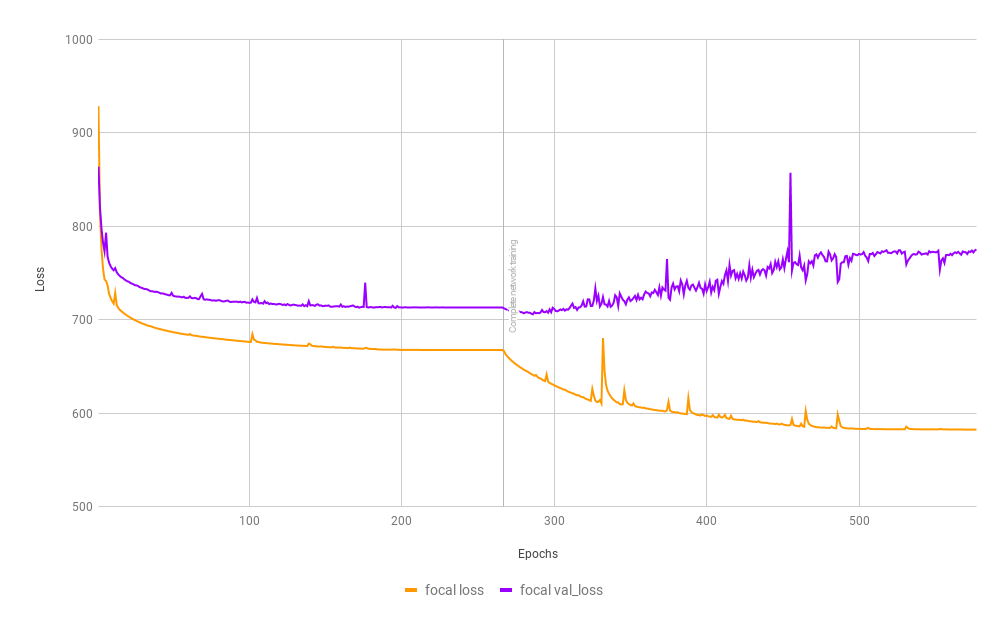
\includegraphics[width=1.\columnwidth]{../imagens/graficos/cap6_bsds_add_focal_morf_v1v2_20200409.png}
%   \caption{Training and validation losses using ALO-ADD/MORPH method on BSDS500.}
%   \label{fig:bsds_add_focal_morf_v1v2}
% \end{figure}

% It can be seen, that the network quickly converged from pre-trained weights.
% After about 130 epochs, the network has stabilized, with small performance gains.
% After no gain for 50 epochs, the protocol ended its first phase.

In second phase of the protocol, the network had a sharp decay in the training loss. %, as can be seen in Figure \ref{fig:bsds_add_focal_morf_v1v2}.
Contrarily, validation loss increased (this condition will be carefully analysed in Section \ref{ssec:basic_pred_eval}).
Close to the 500th epoch, the network showed again poor training loss decrease and it was finished in the 567th epoch.

%--------------------------------
\subsubsection{ALO-AVG}
\label{ssec:bsds_subexp1_avg}

%The second network trained in the protocol was the ALO-AVG, which had similar performance to ALO-ADD in preliminary tests.
The network promptly converged, with a behavior similar to ALO-ADD.
After near 140 epochs, the network has stabilized, with small performance gains. 
The protocol has ended its first phase (only deconvolutions training) at the epoch 219.
%The training and validation losses from steps 1 and 2 of the protocol are shown in Figure \ref{fig:bsds_avg_focal_morf_v1v2}.

% \begin{figure}%[h!]
%   \centering
%   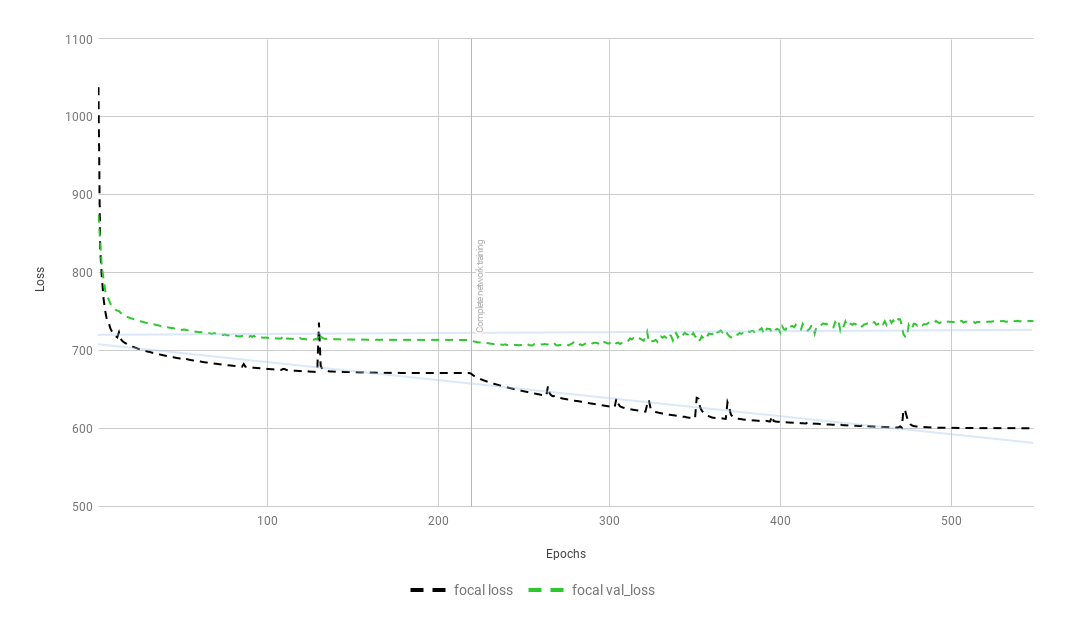
\includegraphics[width=1.\columnwidth]{../imagens/graficos/cap6_bsds_avg_focal_morf_v1v2_20200407.png}
%   \caption{Training and validation losses using ALO-AVG/MORPH method on BSDS500.}
%   \label{fig:bsds_avg_focal_morf_v1v2}
% \end{figure}

% It can be seen in Figure \ref{fig:bsds_avg_focal_morf_v1v2}, that the ALO-AVG promptly converged, with a behavior similar to ALO-ADD.
% After around 140 epochs, the network has stabilized, with small performance gains. 
% The protocol has ended its first phase (only deconvolutions training) at the epoch 219.

In the second phase, the training loss began to decrease slowly, but the validation loss increased, also slowly, for most of the process.
This increase is similar to the training of ALO-ADD, even if it is less than that presented in the previous experiment.
It is important to note that this behavior occurred even with small learning rates (less than $1 \times 10^{-9}$). 

%--------------------------------
\subsubsection{ALO-MAX}
\label{ssec:bsds_subexp1_max}

%ALO-MAX was the last network trained in this experiment.
Contrarily to other networks, ALO-MAX had more difficult to converge properly in preliminary tests.
It had the lowest loss (722.39), 24.06\% more when compared to ALO-ADD (582.29) and 20.29\% more when compared with ALO-AVG (600.54).
%The training and validation losses of ALO-MAX's protocol in phases 1 and 2, the are presented in Figure \ref{fig:bsds_max_focal_morf_v1v2}.

%It can be seen in Figure \ref{fig:bsds_max_focal_morf_v1v2} that the ALO-MAX converged less and slower than the other networks.
%ALO-MAX had the lowest loss (722.39), 24.06\% more when compared to ALO-ADD (582.29) and 20.29\% more when compared with ALO-AVG (600.54).

% \begin{figure}%[h!]
%   \centering
%   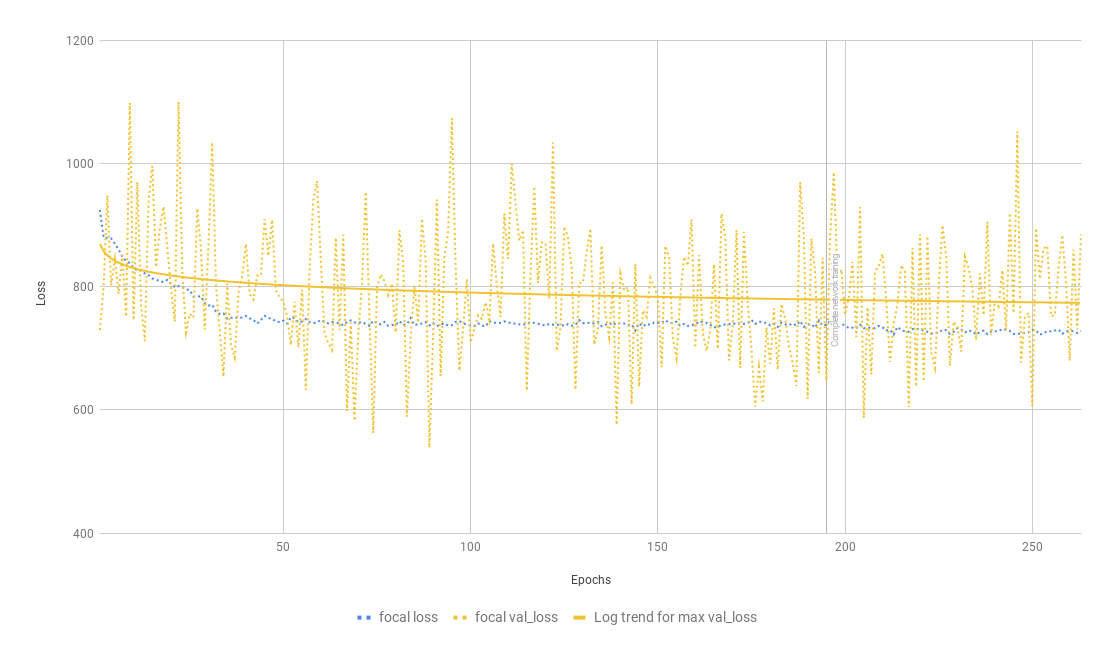
\includegraphics[width=1.\columnwidth]{../imagens/graficos/cap6_bsds_max_focal_morf_v1v2_20200408.png}
%   \caption{Training and validation losses using ALO-MAX/MORPH method on BSDS500.}
%   \label{fig:bsds_max_focal_morf_v1v2}
% \end{figure}

%It is also possible to notice that 
The validation loss was really unstable during both phases, with many ups and downs, without any convergence in the process.
The training was faster than the previous ones, with 94 epochs in the first phase and only 69 epochs in second one.
This behaviour indicates that the network did not improved its results and the training of the deconvolution layers was enough for the network to reach the best possible value.
%It is possible to conclude that only the training of the deconvolution layers was enough for the network to reach the best possible value.

%--------------------------------
% \subsubsection{Networks comparison}
% \label{ssec:bsds_subexp1_comparison}
% 
% To assist in the evaluation of the third phase of the experiments, Figures \ref{fig:bsds_addavgmax_focal_all} and \ref{fig:bsds_addavgmax_focal_upper} with the loss curves were created.
% To aid comparison, the values are presented in a single image, even though the number of training epochs are different for each method.
% Figure \ref{fig:bsds_addavgmax_focal_all} shows training and validation curves for ALL ground truth while Figure \ref{fig:bsds_addavgmax_focal_upper} shows the results for UPPER's.
% 
% \begin{figure}%[h!]
%   \centering
%   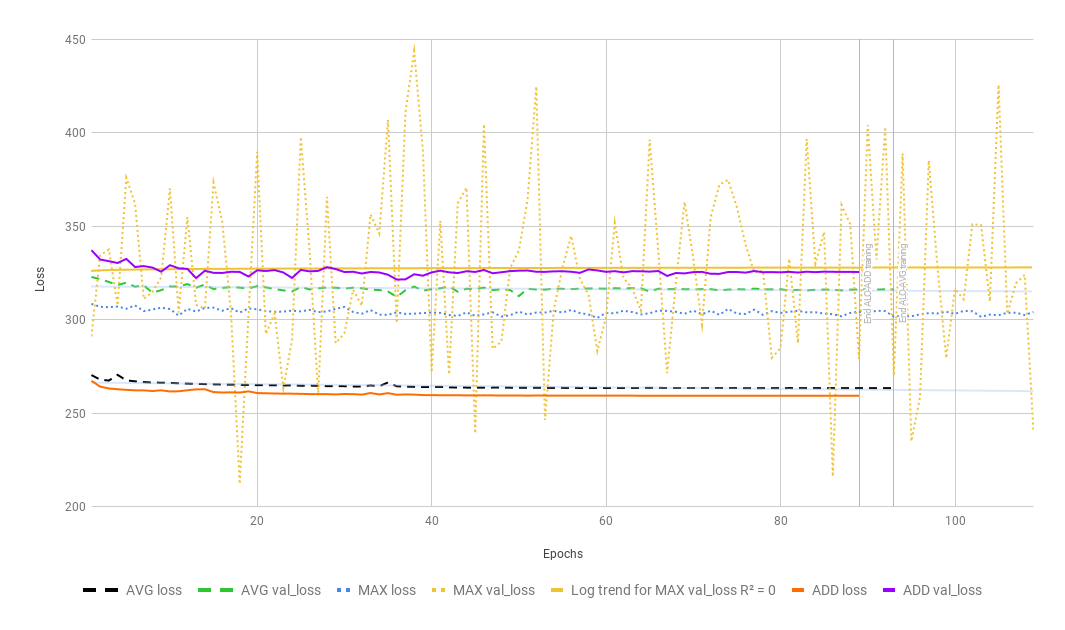
\includegraphics[width=1.\columnwidth]{../imagens/graficos/bsds_addavgmax_focal_all.png}
%   \caption{Loss comparison using ALL ground truth on BSDS500.}
%   \label{fig:bsds_addavgmax_focal_all}
% \end{figure}
% 
% \begin{figure}%[h!]
%   \centering
%   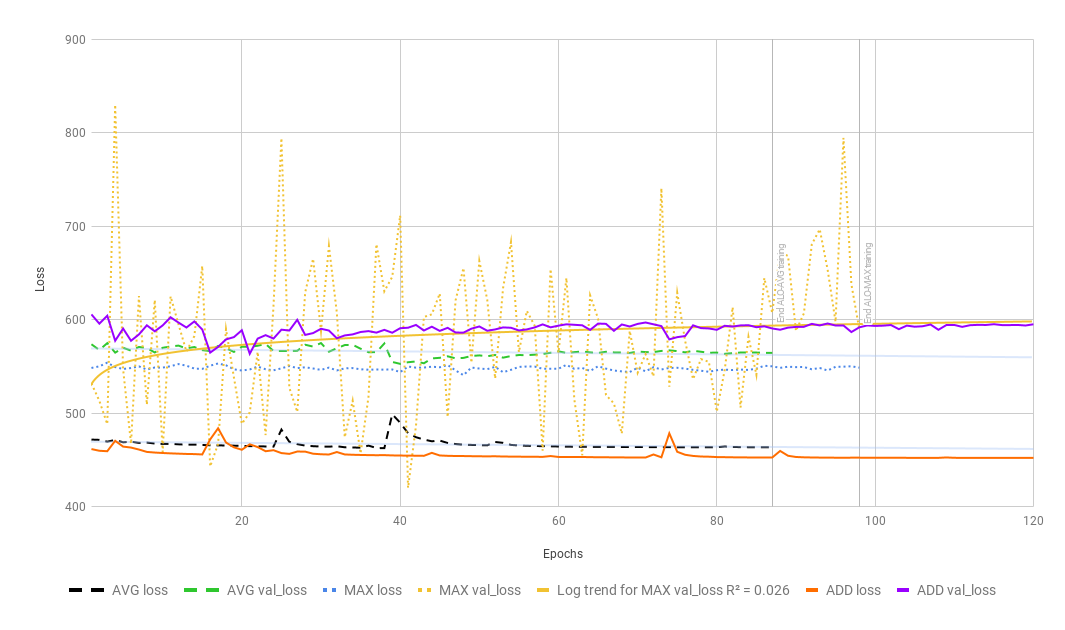
\includegraphics[width=1.\columnwidth]{../imagens/graficos/bsds_addavgmax_focal_upper.png}
%   \caption{Loss comparison using UPPER ground truth on BSDS500.}
%   \label{fig:bsds_addavgmax_focal_upper}
% \end{figure}
% 
% Figure \ref{fig:bsds_addavgmax_focal_all} shows predominantly a small training loss decrease during the entire procedure for the networks.
% In Figure \ref{fig:bsds_addavgmax_focal_upper}, it is possible to observe a higher nominal value of the loss when compared with Figure \ref{fig:bsds_addavgmax_focal_all}, caused by the different ground truth.
% The validation curves for ALO-ADD and ALO-AVG are somewhat unstable at the beginning of the process and becomes more stable throughout the training.
% 
% Figures \ref{fig:bsds_addavgmax_focal_all} and \ref{fig:bsds_addavgmax_focal_upper} shows that ALO-AVG and ALO-ADD had low fluctuation during all training period, without converging to smaller values.
% The gain were really small, indicating that networks are almost training.
% ALO-ADD training loss is smaller than ALO-AVG, but its validation loss was bigger during all training process.
% 
% It is possible to see in Figures \ref{fig:bsds_addavgmax_focal_all} and \ref{fig:bsds_addavgmax_focal_upper} that ALO-MAX presented the same problems as previously described in Section \ref{ssec:bsds_subexp1_max}.
% Validation loss kept unstable with high volatility, in opposite to its training loss.
% Despite the stability, the training loss had high value, making it closer to validation curves from AVG and ADD methods.
% This behavior indicates that the network was not able to generalize well. %, as can be seen in the performance analysis below.

% To complement the information provided by the analysis of losses, a performance evaluation was done using another metric, accuracy, as shown in Figure \ref{fig:bsds_focal_upper_metrics}.
% In there, it can be seen that training accuracy values are closes to 0.96 while validation accuracy is close to 0.9575, indicating that the data augmentation is sufficient for the problem and is also suitable for larger network architectures
% 
% \begin{figure}%[h!]
%   \centering
%   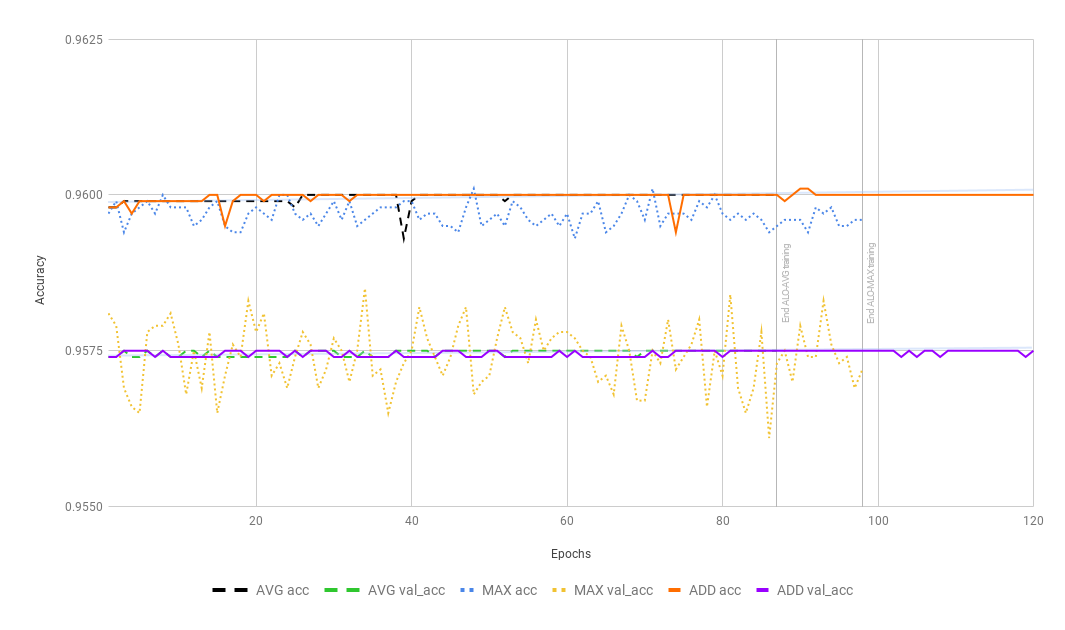
\includegraphics[width=1.\columnwidth]{../imagens/graficos/bsds_focal_upper_metrics.png}
%   \caption{Accuracy comparison using UPPER ground truth on BSDS500.}
%   \label{fig:bsds_focal_upper_metrics}
% \end{figure}
% 
% Figure \ref{fig:bsds_focal_upper_metrics} also indicates that ALO-MAX had close values to other methods, despite low performance in loss metrics.
% This can be explained due the number of background pixels in the image, making accuracy an inappropriate metric to evaluate the results.

\begin{comment}
Once the objective functions are different, it's not possible to compare metrics values returned by training statistics in each phase. 
For this, it was evaluated the results of border detection using BSDS500 Benchmark.
The results will be shown in Section \ref{ssec:basic_pred_eval}, when they will be compared to the results obtained by the ALO-AVG and ALO-MAX networks, that will be described in the following sections.
\end{comment}

%--------------------------------
\subsection{Evaluation and Predictions}
\label{ssec:basic_pred_eval}

Due to the low capacity to evaluate the previous experiments using the accuracy metric, it was decided to evaluate the model with BSDS500 Benchmark.
The results are presented in Figure \ref{fig:bsds_subexp1_results}. %Table \ref{tab:bsds_subexp1_results}.
To evaluate the gain of UPPER and ALL ground truths usage, it was decided to evaluate MORPH performance also.
As explained in Section \ref{ssec:framework_experiments}, the network was trained until it does not improve for 50 epochs, making MORPH almost unable to perform better.

% \begin{table}%[h!]
%   \centering
%   \caption{Border detection performance on BSDS500 for ALO-AVG, ALO-ADD and ALO-MAX.}
%   \scriptsize
%   %\setlength{\tabcolsep}{1em}
%   \renewcommand{\arraystretch}{1.5}
%   \begin{tabular}{{c}{c}{c}{c}{c}{c}{c}}
%     \hline
%     Network & Loss & Ground truth & TH & ODS & OIS %& Area PR
%     \\
%     \hline
%     ALO-ADD & FL & MORPH (v1) & 0.51 & 0.7214 & 0.7461 %& 0.4721
%     \\
%     ALO-ADD & FL & MORPH (v2) & 0.50 & 0.7376 & 0.7596 %& 0.5331
%     \\
%     ALO-ADD & FL & ALL & 0.40 & 0.7504 & \textbf{0.7714} %& 0.6105
%     \\
%     ALO-ADD & FL & UPPER & 0.47 & \textbf{0.7512} & 0.7704 %& 0.5809
%     \\
%     ALO-AVG & FL & MORPH (v1) & 0.52 & 0.7227 & 0.7462 %& 0.4862
%     \\
%     ALO-AVG & FL & MORPH (v2) & 0.51 & 0.7384 & 0.7606 %& 0.5356
%     \\
%     ALO-AVG & FL & ALL & 0.40 & 0.7496 & 0.7708 %& 0.5932
%     \\
%     ALO-AVG & FL & UPPER & 0.46 & 0.7500 & 0.7690 %& 0.5796
%     \\
%     \hline
%     ALO-MAX & FL & MORPH (v1) & 0.70 & 0.6911 & 0.7127 %& 0.5712
%     \\
%     ALO-MAX & FL & MORPH (v2) & 0.67 & 0.7039 & 0.7247 %& 0.5510
%     \\
%     ALO-MAX & FL & ALL & 0.56 & 0.7122 & 0.7311 %& \textbf{0.6337}
%     \\
%     ALO-MAX & FL & UPPER & 0.64 & 0.7127 & 0.7326 %& 0.5932
%     \\
%     \hline
%   \end{tabular}
%   \label{tab:bsds_subexp1_results}
% \end{table}

\begin{figure*}%[h!]
  \centering
  %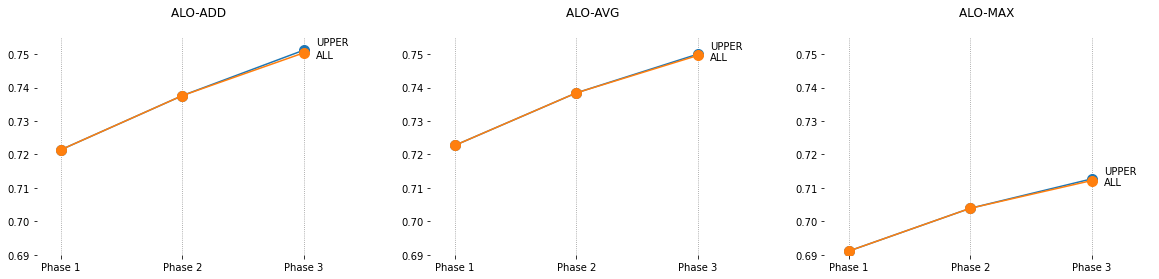
\includegraphics[width=0.8\textwidth]{../imagens/visualiz_dados/bsds_experiment_2-1.png}
  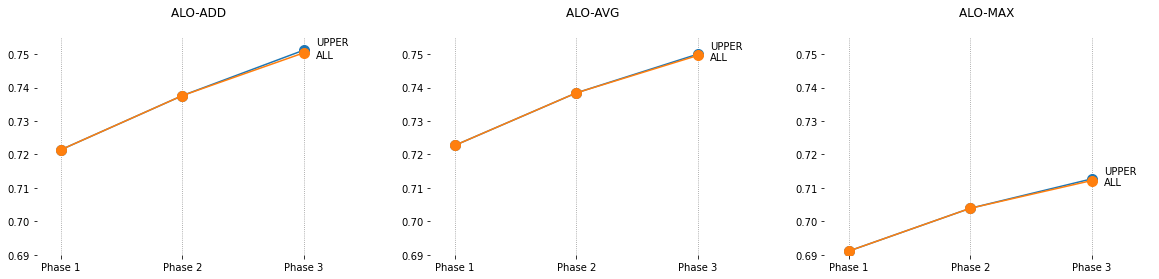
\includegraphics[width=1\textwidth]{../imagens/visualiz_dados/bsds_experiment_2-1.png} %VISUALIZ
  \caption{Border detection ODS performance on BSDS500 for ALO-AVG, ALO-ADD and ALO-MAX in Experiment 1.}
  \label{fig:bsds_subexp1_results}
\end{figure*}

\begin{comment}
Figure \ref{fig:bsds_subexp1_results} was developed using small multiples technique to show the difference between methods.
ALO-ADD and ALO-AVG were plotted in different images once the results were similar and one data was above other.
This results contrasts with the poor performance of ALO-MAX network.
\end{comment}

The overall results of ALO-ADD and ALO-AVG were really similar, considerably better than ALO-MAX. %but ALO-ADD had better performance using both ODS and OIS metrics.
The number of training epochs to reach the best results were also similar, as described in Table \ref{tab:bsds_subexp1_epochs}. %, but with less epochs for ALO-AVG.
These results indicates that both methods are similar in performance and number of training epochs.
%Table \ref{tab:bsds_subexp1_epochs} also shows that 
In contrast, ALO-MAX had the least number of training epochs.
However, due to its poor performance, this information cannot be used in favor of the method.

%It is possible to notice, in the analysis of Table \ref{tab:bsds_subexp1_results}, that all networks improved with training using ALL or UPPER ground truths.
It is also possible to notice, in the analysis of Figure \ref{fig:bsds_subexp1_results}, that all networks improved with training using ALL or UPPER ground truths.
The benefit of using both ground truths is around 1,5\% in comparison with the best result achieved by MORPH ground truth.


% Using the analysis of Figures \ref{fig:bsds_addavgmax_focal_all} and \ref{fig:bsds_addavgmax_focal_upper}, it is important to remember that these networks have barely improved their performance in the last phase of the protocol.

These results can be partially explained due to the deformation caused by the morphological thinning operation.
UPPER and ALL ground truths maintains the original outline of the edges.
Also, the differences can be seen as just an adjust of the weights, to provide hard and soft defined borders.
This difference seems to influence the evaluation, once the benchmark compare borders with each human annotation in each ground truth.

\begin{comment}
It is also important to notice in Table \ref{tab:bsds_subexp1_results} that ALL and UPPER ground truths reduced the thresholds for the OIS and ODS values.
Once the threshold it is smaller than 0.5, this mean, in a binary way, that some borders are most similar to the background than the border class.
These borders just was plotted in the image because the values were presented in a scale of confidence, ignoring the most probable class.
When the MORPH ground truth was used, all classes were above 0.5, indicating that the results were well defined, despite the lower final result than those obtained with other ground truths.
\end{comment}

\begin{table}%[h!]
  \centering
  \caption{Number of training epochs in Experiment 2.1.}
  %\scriptsize
  %\setlength{\tabcolsep}{1em}
  \renewcommand{\arraystretch}{1.5}
  \begin{tabular}{{c}{c}{c}{c}{c}{c}{c}}
    \hline
    Ground truth & ALO-ADD & ALO-AVG & ALO-MAX
    \\
    \hline
    MORPH / ALL & 666 & 641 & 372
    \\
    MORPH / UPPER & 697 & 635 & 361
    \\
    \hline
  \end{tabular}
  \vspace{0.2cm}
  \label{tab:bsds_subexp1_epochs}
\end{table}

%To complete the information about training, it is important to view the visual results of the methods.
%These results are available in Figure \ref{fig:cap6_expr1_bsds_visual}, with the original prediction and with the best threshold cut, informed by the BSDS500 benchmark.

% \begin{figure*}
%   \centering
%   \captionsetup[subfigure]{labelformat=empty}
%   \subfloat[BSDS500 image\label{fig:cap6_expr1_img}]{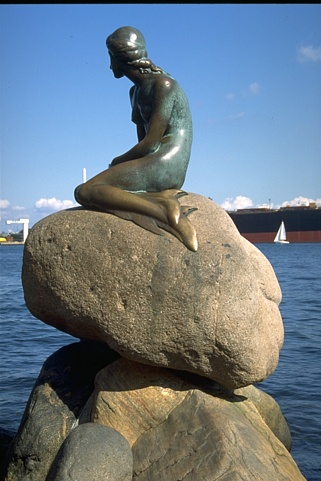
\includegraphics[width=0.24\textwidth]{../imagens/ilustracoes/cap6_bsds_372019.jpg}}
%   \hfill
%   \subfloat[ALO-ADD\label{fig:cap6_expr1_add}]{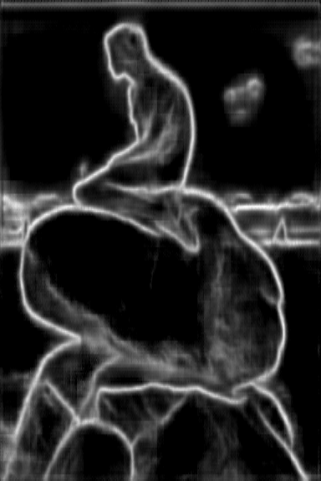
\includegraphics[width=0.24\textwidth]{../imagens/ilustracoes/cap6_bsds_372019_add_20200409.png}}
%   \hfill
%   \subfloat[ALO-AVG\label{fig:cap6_expr1_avg}]{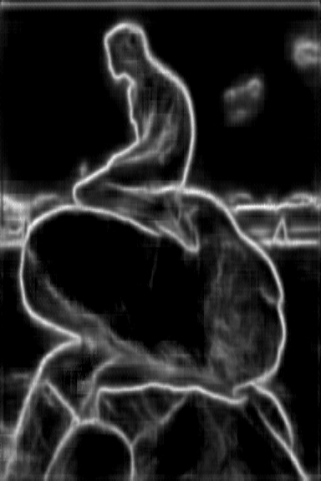
\includegraphics[width=0.24\textwidth]{../imagens/ilustracoes/cap6_bsds_372019_avg_20200407.png}}
%   \hfill
%   \subfloat[ALO-MAX\label{fig:cap6_expr1_max}]{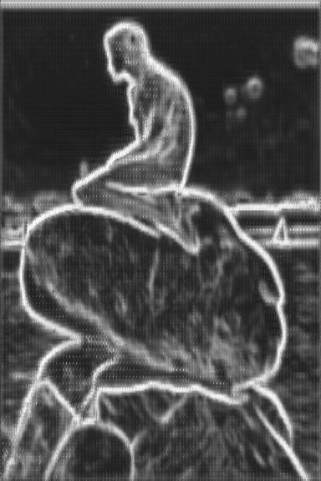
\includegraphics[width=0.24\textwidth]{../imagens/ilustracoes/cap6_bsds_372019_max_20200408.png}}
%   %\caption{Original image (a) and it borders detected by ALO-ADD (b), ALO-AVG (c) and ALO-MAX (d), using MORPH/UPPER ground truth methods.}
%   
%   \subfloat[Ground truth\label{fig:cap6_expr1_gt}]{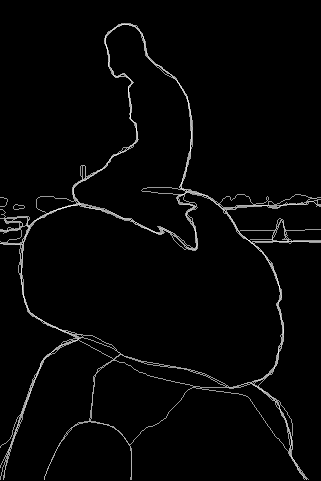
\includegraphics[width=0.24\textwidth]{../imagens/html/372019_upper.png}}
%   \hfill
%   \subfloat[ALO-ADD (0.47)\label{fig:cap6_expr1_add_th}]{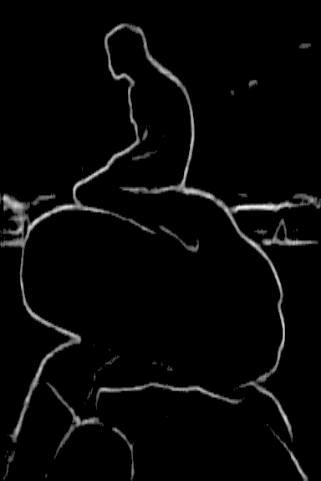
\includegraphics[width=0.24\textwidth]{../imagens/ilustracoes/cap6_bsds_372019_add_20200409_047.png}}
%   \hfill
%   \subfloat[ALO-AVG (0.46)\label{fig:cap6_expr1_avg_th}]{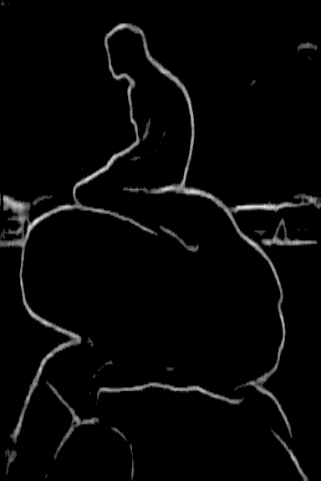
\includegraphics[width=0.24\textwidth]{../imagens/ilustracoes/cap6_bsds_372019_avg_20200407_046.png}}
%   \hfill
%   \subfloat[ALO-MAX (0.64)\label{fig:cap6_expr1_max_th}]{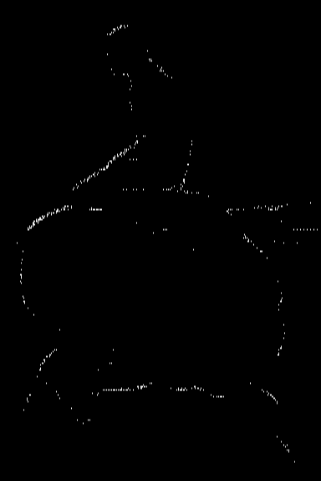
\includegraphics[width=0.24\textwidth]{../imagens/ilustracoes/cap6_bsds_372019_max_20200408_064.png}}
%   \caption{Predictions of the ALO-ADD, ALO-AVG and ALO-MAX networks, and its best thresholds.}
%   \label{fig:cap6_expr1_bsds_visual}
% \end{figure*}

%Figure \ref{fig:cap6_expr1_bsds_visual} shows that the predictions of ALO-ADD and ALO-AVG are quite similar, corroborating the results in Table \ref{tab:bsds_subexp1_results}.
%Also, the results shows that ALO-MAX didn't performed well, once it contains a lot of noise.
%Its best threshold removed many border details, resulting only in sparse pixels following the expected shape, but without producing a contour.

After this experiment, it was decided that the ALO-MAX method will no longer be tested, due to its low performance and weak convergence. %\footnote{ALO-MAX also had poor performance in preliminary experiments.}.
The following sections will provide and discuss experiments using only the ALO-ADD and ALO-AVG methods.

%--------------------------------
\subsection{Experiment 2.2 - Improving Focal Loss and Hyperparameter Tuning}
\label{ssec:bsds_subexp2}

After training BSDS500 using Focal Loss, a new experiment was developed to try to increase the results achieved and decrease the number of training epochs.
To do it, a simple change in Focal Loss is proposed in this section.
The suggested change is to add the metric Pixel-Error (PE), as a factor to improve Focal Loss (FL).

The purpose of the modification is to increase the separation between the edges and the background, making the network convergence faster.
It is important to clarify that this change will mainly affect the ground truths MORPH and UPPER, that contains edge values far from background values.
The new metric, named PEFL (\textit{Pixel-Error Focal Loss}), can be simple defined as Equation \ref{equ:pixel_error_focal_loss}:

\begin{equation}
  PEFL = FL \times (1 + PE)
  \label{equ:pixel_error_focal_loss}
\end{equation}

In conjunction with the new loss function, some hyper-parameter tuning were made\footnote{~The experiment described in Section \ref{ssec:bsds_subexp1} was performed again, changing only the loss function. It produced, using ALL and UPPER ground truths, 0.7502 and 0.7505 ODS values, with 429 (36\% less) and 460 (34\% less) epochs, respectively.}.
Some quick experiments were carried out and the one that showed the greatest evidence of improvement was the reduction in \textit{gamma} parameter.
Then, ALO-ADD and ALO-AVG networks were fully trained with the following changes in default parameterization, defined in Section \ref{ssec:framework_experiments}.

\begin{center}
Loss: PEFL ($\gamma$=1.0; $\alpha$=0.25)
\end{center}

% For the new experiment, the learning curves for MORPH phases are available in Figure \ref{fig:bsds_avg_fuse_1_morf}.
% It is noteworthy that ALO-AVG had, in all phases, a similar behavior to the network ALO-MAX in the experiment described in Section \ref{ssec:bsds_subexp1}.
% This unusual behavior, nonetheless, did not increase the number of training epochs nor decrease the performance.
% 
% \begin{figure}%[h!]
%   \centering
%   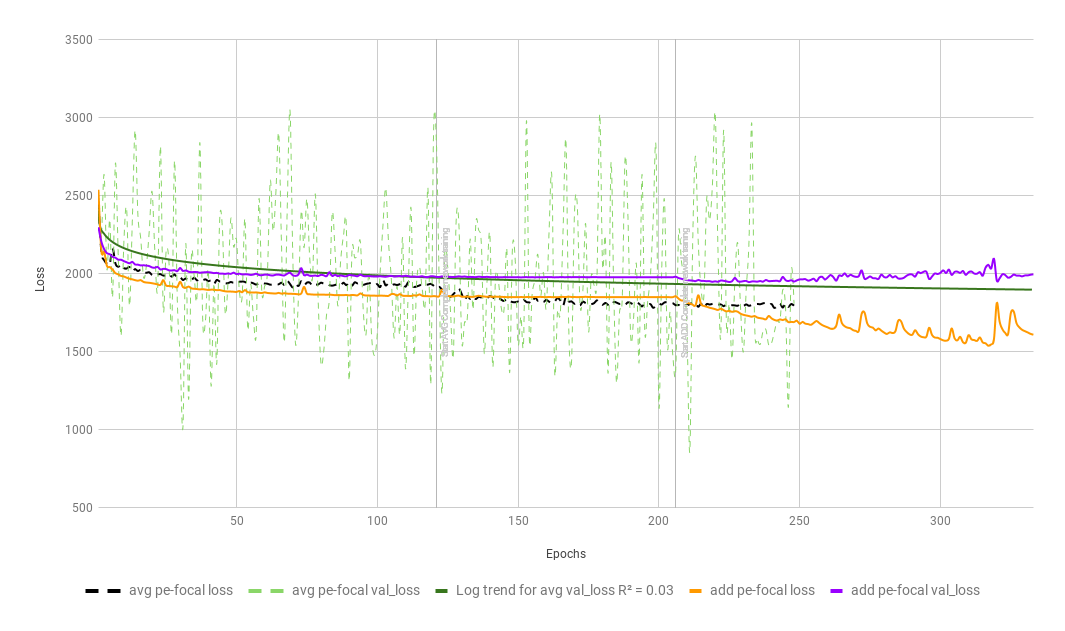
\includegraphics[width=1.\columnwidth]{../imagens/graficos/cap6_bsds_fuse_morf_v1v2_20200410-20.png}
%   \caption{Training and validation losses of ALO-ADD and ALO-AVG methods on BSDS500, using MORPH ground truth.}
%   \label{fig:bsds_avg_fuse_1_morf}
% \end{figure}

In the new experiment, ALO-AVG had, in all phases, a similar behavior to the network ALO-MAX in the experiment described in Section \ref{ssec:bsds_subexp1}.
This unusual behavior, nonetheless, did not increase the number of training epochs nor decrease the performance.
Instead, it performed better than that obtained in the experiment described in Section \ref{ssec:bsds_subexp1}, using the default parameterization, as can be seen in Table \ref{tab:bsds_subexp2_results}.

% The benchmark evaluation of ALO-AVG and ALO-ADD performances are available in Table \ref{tab:bsds_subexp2_results}.
% The number of training epochs are presented in Table \ref{tab:bsds_subexp2_epochs}.

\begin{table}%[h!]
  \centering
  \caption{Border detection performance on BSDS500 for ALO-ADD and ALO-AVG in Experiment 2.2.}
  %\scriptsize
  %\setlength{\tabcolsep}{1em}
  \renewcommand{\arraystretch}{1.5}
  \begin{tabular}{{c}{c}{c}{c}{c}{c}{c}}
    \hline
    Network & Loss & Ground truth & TH & ODS & OIS %& Area PR
    \\
    \hline
    ALO-ADD & PEFL & ALL & 0.21 & 0.7558 & \textbf{0.7776} %& 0.6717
    \\
    ALO-ADD & PEFL & UPPER & 0.30 & 0.7559 & 0.7746 %& 0.6561
    \\
    \hline
    ALO-AVG & PEFL & ALL & 0.20 & 0.7546 & 0.7770 %& 0.6790
    \\
    ALO-AVG & PEFL & UPPER & 0.30 & \textbf{0.7563} & 0.7749 %& 0.673
    \\
    \hline
  \end{tabular}
  \label{tab:bsds_subexp2_results}
\end{table}

\begin{table}%[h!]
  \centering
  \caption{Number of training epochs in Experiment 2.2.}
  %\scriptsize
  %\setlength{\tabcolsep}{1em}
  \renewcommand{\arraystretch}{1.5}
  \begin{tabular}{{c}{c}{c}{c}{c}{c}{c}}
    \hline
    Ground truth & ALO-ADD & ALO-AVG 
    \\
    \hline
    MORPH / ALL & 553 & 409
    \\
    MORPH / UPPER & 620 & 473
    \\
    \hline
  \end{tabular}
  \label{tab:bsds_subexp2_epochs} 
\end{table}

Table \ref{tab:bsds_subexp2_epochs}  shows that the number of training epochs has decreased compared to the results of the previous training, available in Table \ref{tab:bsds_subexp1_epochs}.
Comparing the number of epochs of both experiments, it is possible to perceive that ALO-ADD reduced 16.97\% in MORPH/ALL method and 11.05\% in MORPH/UPPER method.
ALO-AVG performed even better, with reduction of training epochs for MORPH/ALL 36.19\% and 25.51\% for MORPH/UPPER ground truths.
It is important to remember that both networks have increased their performance when compared to previous experiments.

%--------------------------------
\subsection{Side-Outputs Contribution}
\label{ssec:bsds_sideout}

After training the network in previous experiments, it is important to evaluate the contributions of each layer.
Model interpretation can help decision making process to obtain knowledge to improve the model's performance \cite{Hohman:2019} and, also, improve results trustworthiness \cite{Chatzimparmpas:2020}.
%Contrary to what was done in Section \ref{cap6_contribuicoes_saidas_intermediarias}, where only the last layer of each stage was plotted, Figures \ref{fig:bsds_add_side_outputs} and \ref{fig:bsds_avg_side_outputs} displays information for all side-outputs of the networks.

%Contrary to what was done in Section \ref{cap6_contribuicoes_saidas_intermediarias}, where only the last layer of each stage was plotted,
Figure \ref{fig:bsds_stage_outputs} combine results from side-outputs inside one distinct stage while Figure \ref{fig:bsds_stage_results} combine results of all previous stages, until the current one.
Figure \ref{fig:bsds_stage_outputs} helps to understand how each stage combine to the final output while \ref{fig:bsds_stage_results} helps to evaluate the gain when some stages are added to the final output.
Both images can contribute to the evaluation of a possible removal of stages in the network architecture.

% Then, Figure \ref{fig:bsds_stage_outputs} helps to understand how each stage combine to the final output while \ref{fig:bsds_stage_results} helps to evaluate the gain when some stages are added to the final output.
% Both images can contribute to the evaluation of a possible removal of stages in the network architecture.

% \begin{figure}%[h!]
%   \centering
%   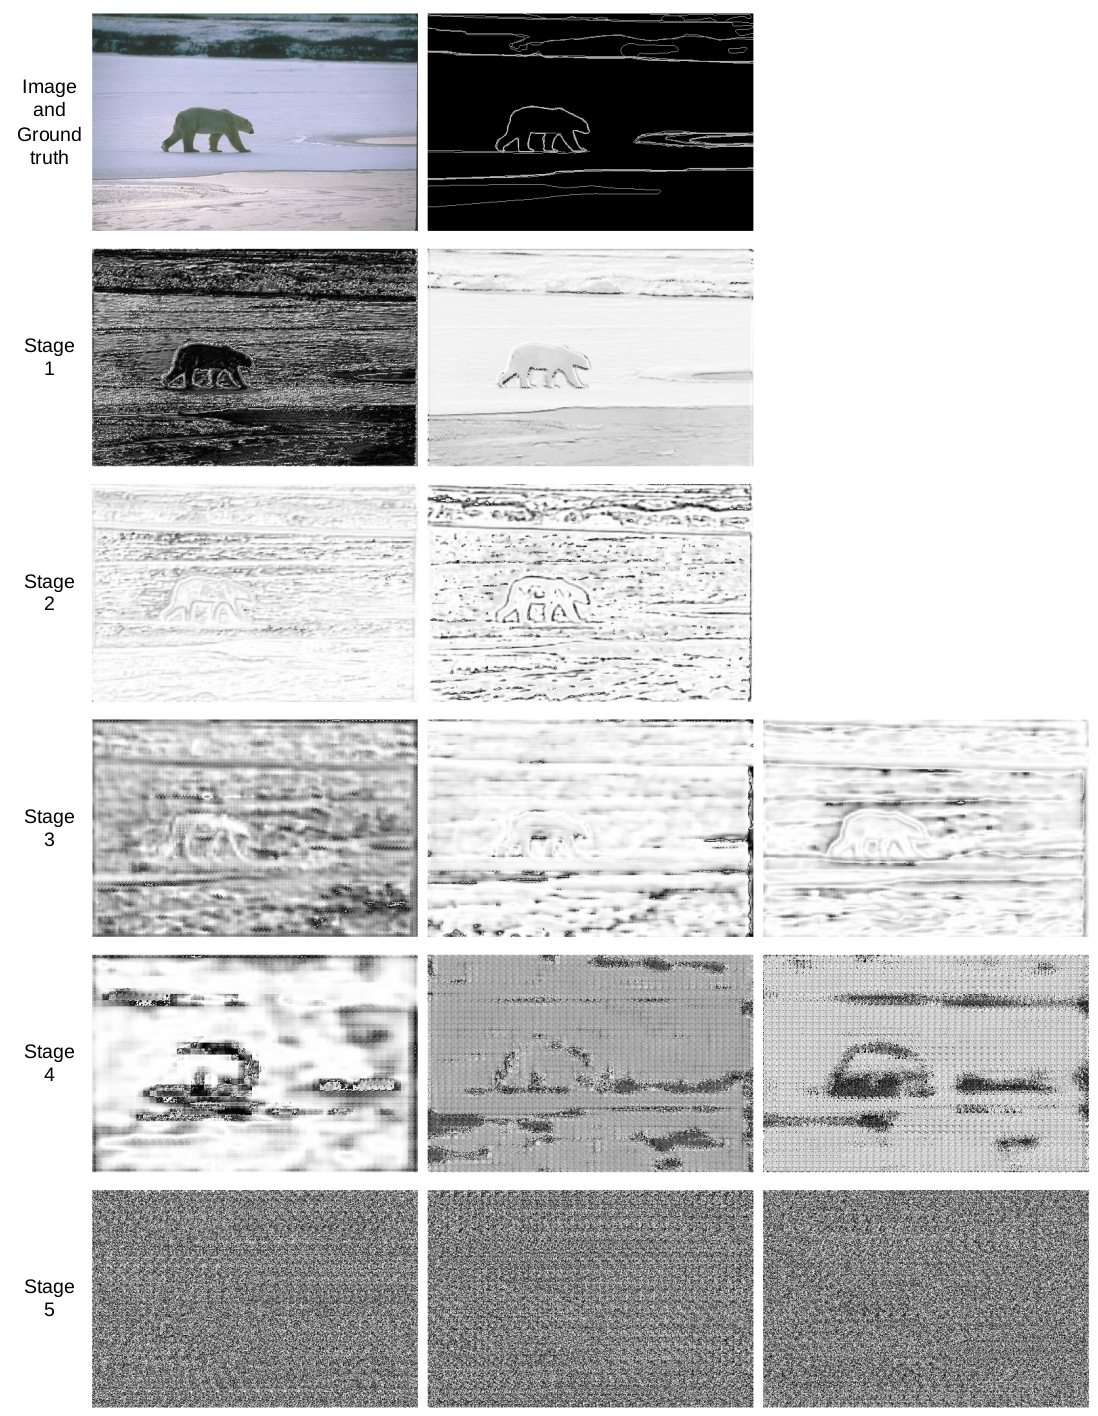
\includegraphics[width=1\columnwidth]{../imagens/ilustracoes/cap6_bsds_add_side_outputs.png}
%   \caption{Side-outputs of each convolution of ALO-ADD method, trained with BSDS 500 using MORPH/UPPER ground truth methods.}
%   \label{fig:bsds_add_side_outputs}
% \end{figure}
% 
% \begin{figure}%[h!]
%   \centering
%   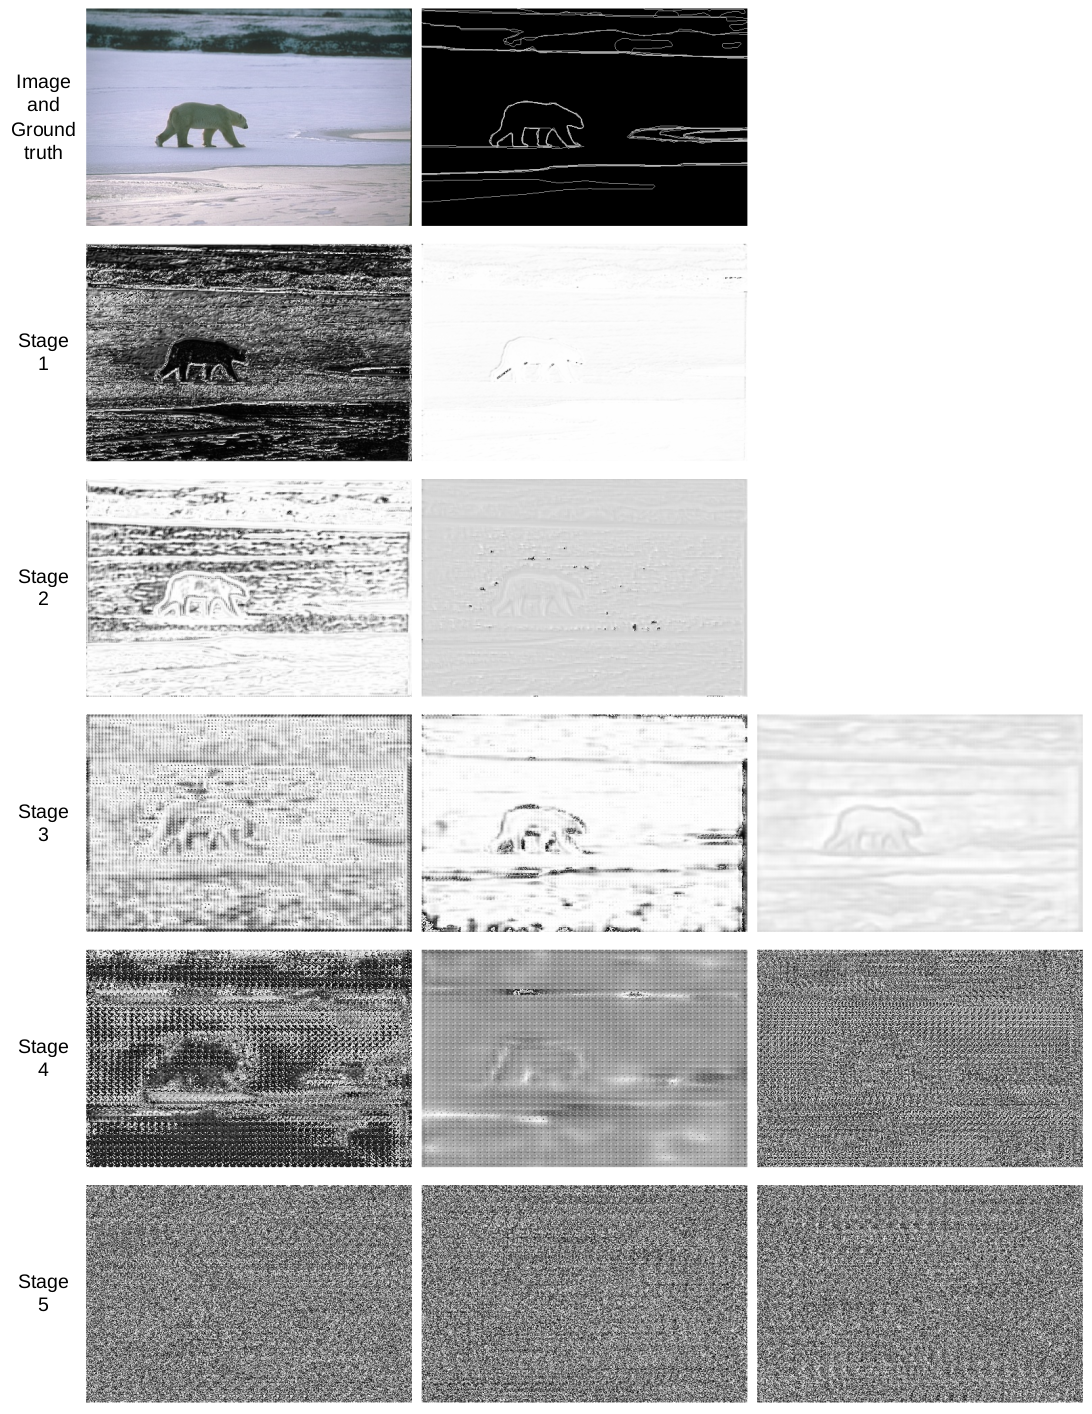
\includegraphics[width=1\columnwidth]{../imagens/ilustracoes/cap6_bsds_avg_side_outputs.png}
%   \caption{Side-outputs of each convolution of ALO-AVG method, trained with BSDS 500 using MORPH/UPPER ground truth methods.}
%   \label{fig:bsds_avg_side_outputs}
% \end{figure}

% It can be seen, in Figures \ref{fig:bsds_add_side_outputs} and \ref{fig:bsds_avg_side_outputs}, that the side-outputs of the first three stages are able to better identify the edges than the outputs of the final stages.

It can be seen, in Figures \ref{fig:bsds_stage_outputs} and \ref{fig:bsds_stage_results}, that the side-outputs of the first three stages are able to better identify the edges than the outputs of the final stages.
The last two stages only assist the results presented by the initial layers, and the latest one, in both networks, does not seen to have any important information for the network, only random noises.

It is also important to notice in Figure \ref{fig:bsds_stage_outputs} that most layers exhibit a large amount of light pixels (borders) compared to dark pixels (background).
This behavior can be considered unexpected, as the final result has borders and backgrounds in the correct colors and tones.
However, it is possible to see that the border, in most of them, is lighter than the surrounding colors, indicating an border.
Also, it was observed that the latest convolution, with operation of $1 \times 1$, described in Section \ref{cap5_saida_final_rede}, helps to separate these colors and tones, making the result close to the ground truth.

% Looking specifically at the first stage, with the assistance of Figures \ref{fig:bsds_add_side_outputs} and \ref{fig:bsds_avg_side_outputs}, it is noticed that both networks presents the same behavior.
% The first output present, in both networks, a dark image with general contours of the main object in the scene (a bear).
% Also, contains some noise, mainly in the background (ice/snow).
% The second outputs, contains the opposite characteristics, with an light image and some contours.
% ALO-ADD's second output shows better contours than those of the ALO-AVG, which presents low level of details.

% In the second stage, it is possible to see some differences to the first one.
% The image are clear, with more distinction of regions, due to color change.
% The images contains some noise, but in less quantity than observed in the first stage.
% ALO-AVG second output of this stage presents an image with few distinction between elements, in contrast to the other stage outputs in both networks.

% The third stage contains different results from ALO-ADD and ALO-AVG.
% ALO-ADD presents worse results than the first two stages, especially in the first and second side-output.
% The last output is the best of this stage, but it seems to be worse than the results of the previous stages, in terms of details.
% The first two outputs of ALO-AVG can be compared to those of ALO-ADD, with low performance .
% However, the last output has possibly the best result of all analyzed ALO-AVG side-outputs.

% It is possible to see in Figures \ref{fig:bsds_add_side_outputs} and \ref{fig:bsds_avg_side_outputs} that the last two stages has small contribution to the final output, when compared to the previous ones.
% The fourth stage contains results with little precision, showing only blots in some regions of interest.
% The fifth stage shows only random noises, which probably have little help in improving the results.

% Help to evaluate the results produced by the side-outputs when combined, are presented Figures \ref{fig:bsds_stage_outputs} and \ref{fig:bsds_stage_results}.
% Figure \ref{fig:bsds_stage_outputs} combine results from side-outputs inside one distinct stage while Figure \ref{fig:bsds_stage_results} combine results of all previous stages, until the current one.
% Then, Figure \ref{fig:bsds_stage_outputs} helps to understand how each stage combine to the final output while \ref{fig:bsds_stage_results} helps to evaluate the gain when some stages are added to the final output.
% Both images can contribute to the evaluation of a possible removal of stages in the network architecture.

\begin{figure}%[h!]
  \centering
  %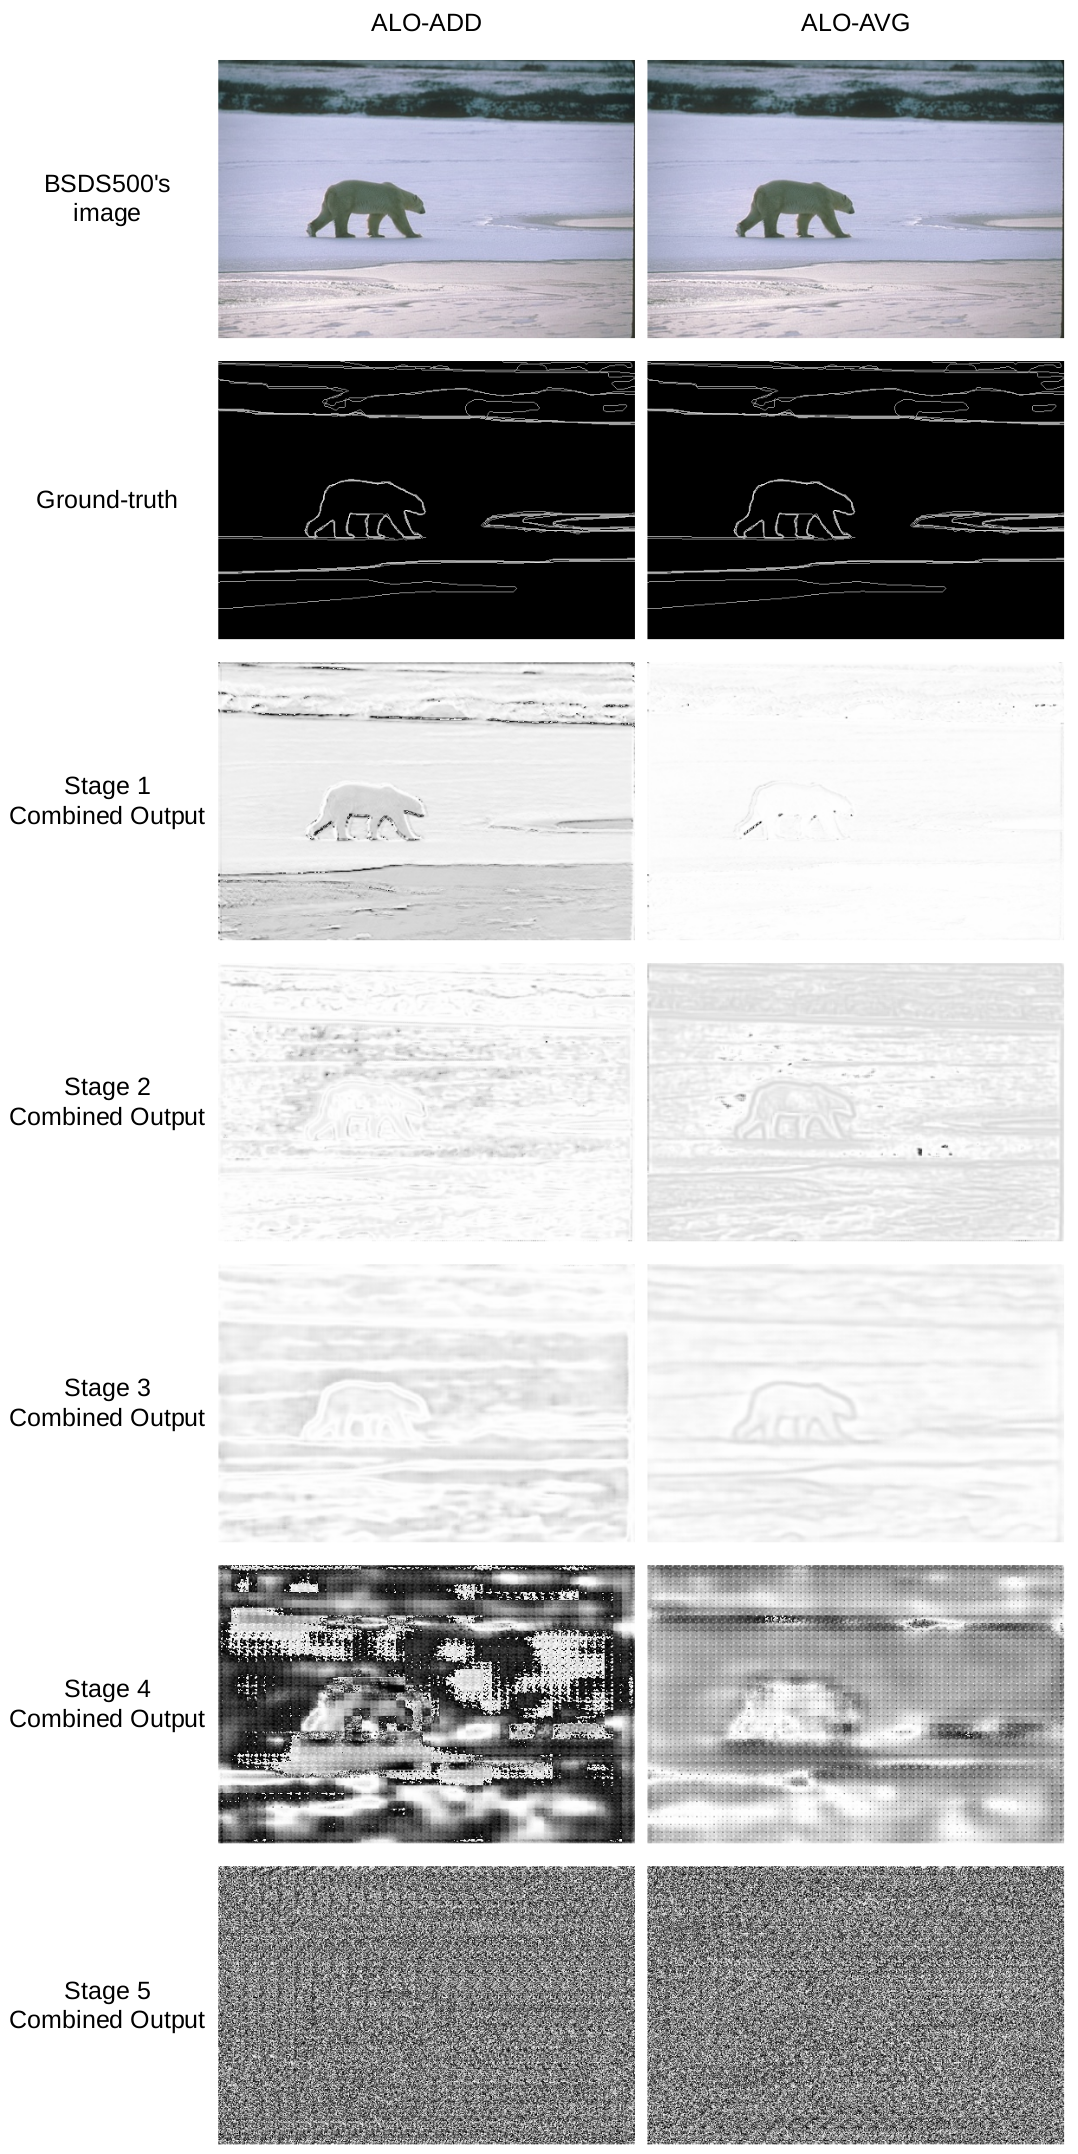
\includegraphics[width=0.9\columnwidth]{../imagens/ilustracoes/cap6_bsds_stage_outputs.png}
  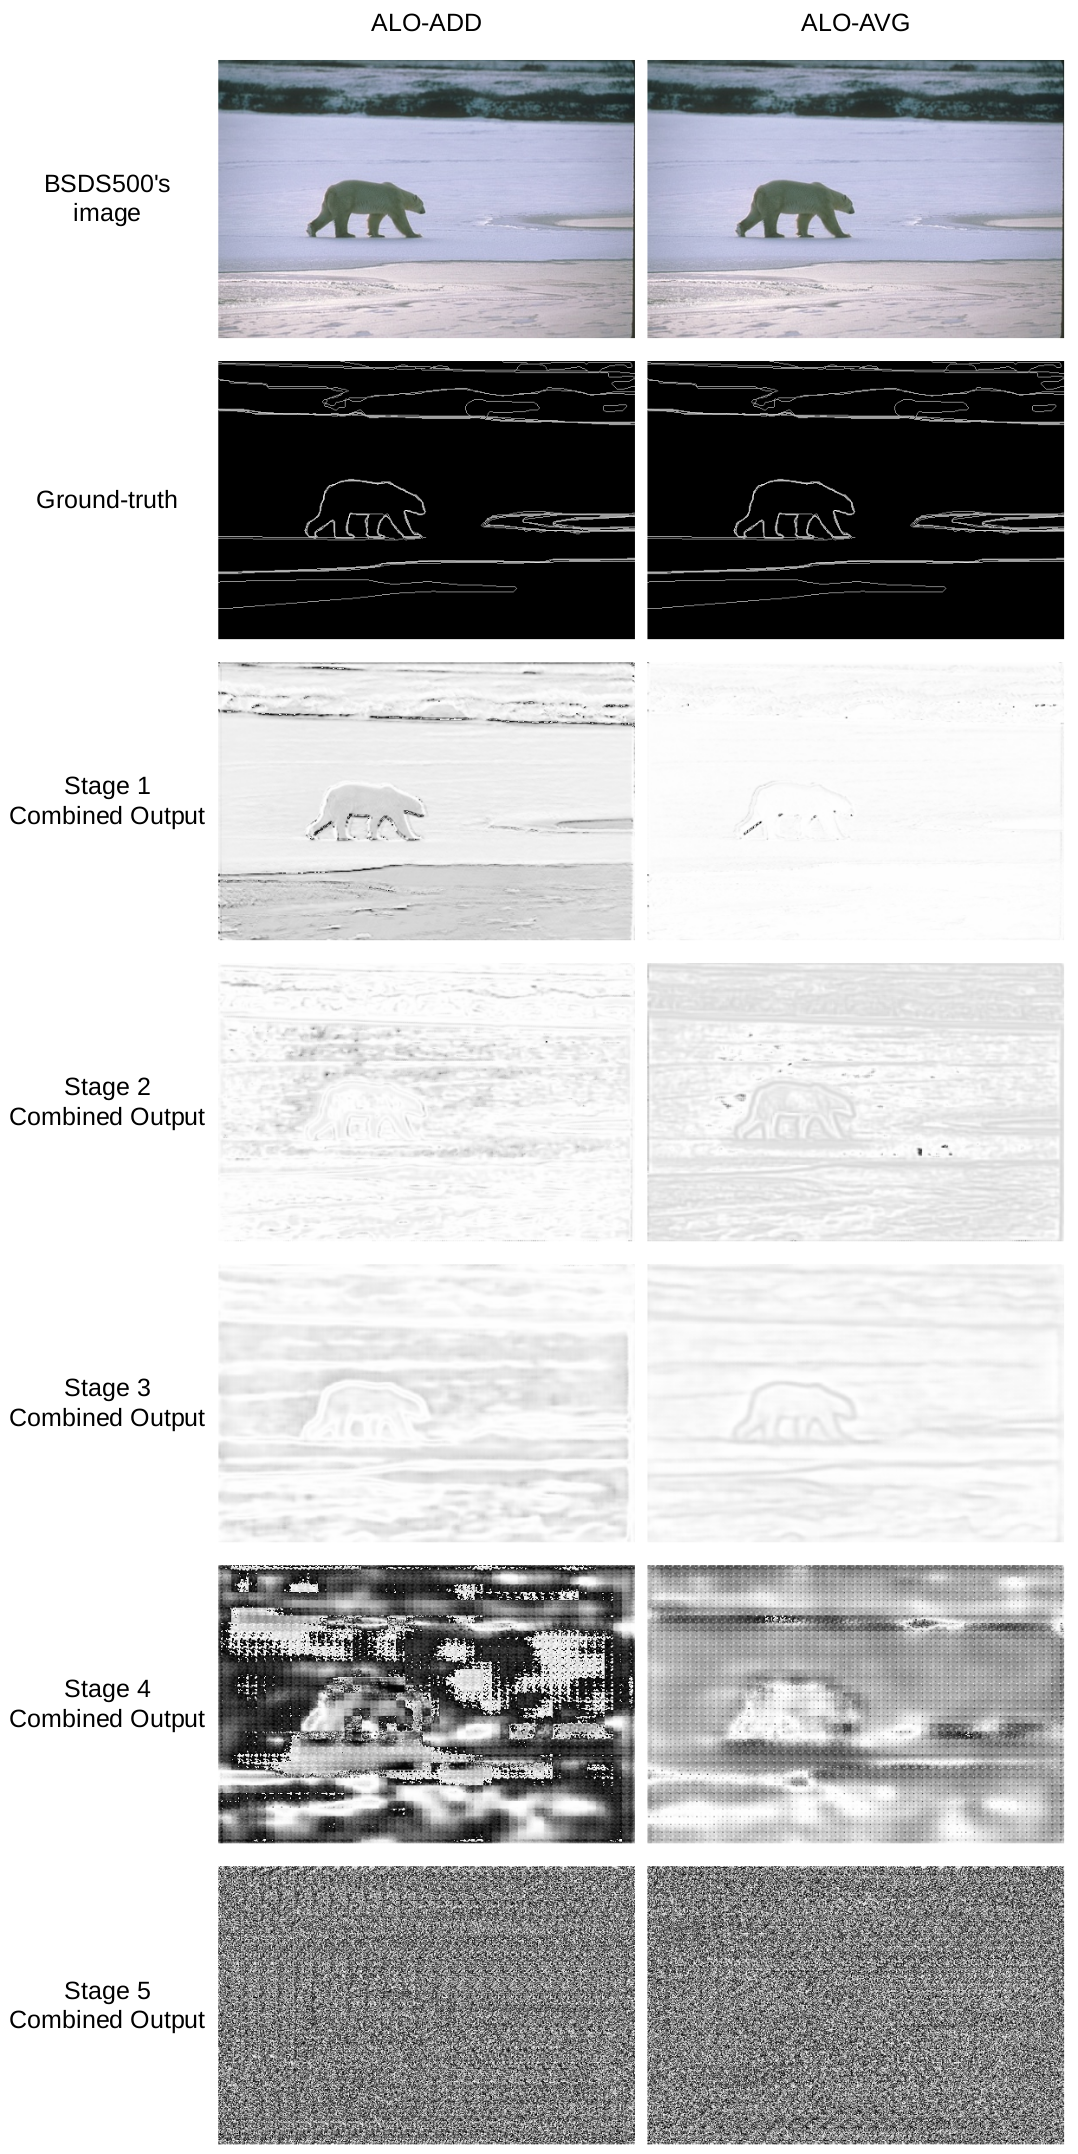
\includegraphics[width=1\columnwidth]{../imagens/ilustracoes/cap6_bsds_stage_outputs.png} %VISUALIZ
  \caption{Side-outputs of each stage of ALO-ADD and ALO-AVG methods, trained with BSDS 500 using MORPH/UPPER ground truth methods.}
  \label{fig:bsds_stage_outputs}
\end{figure}

\begin{figure}%[h!]
  \centering
  %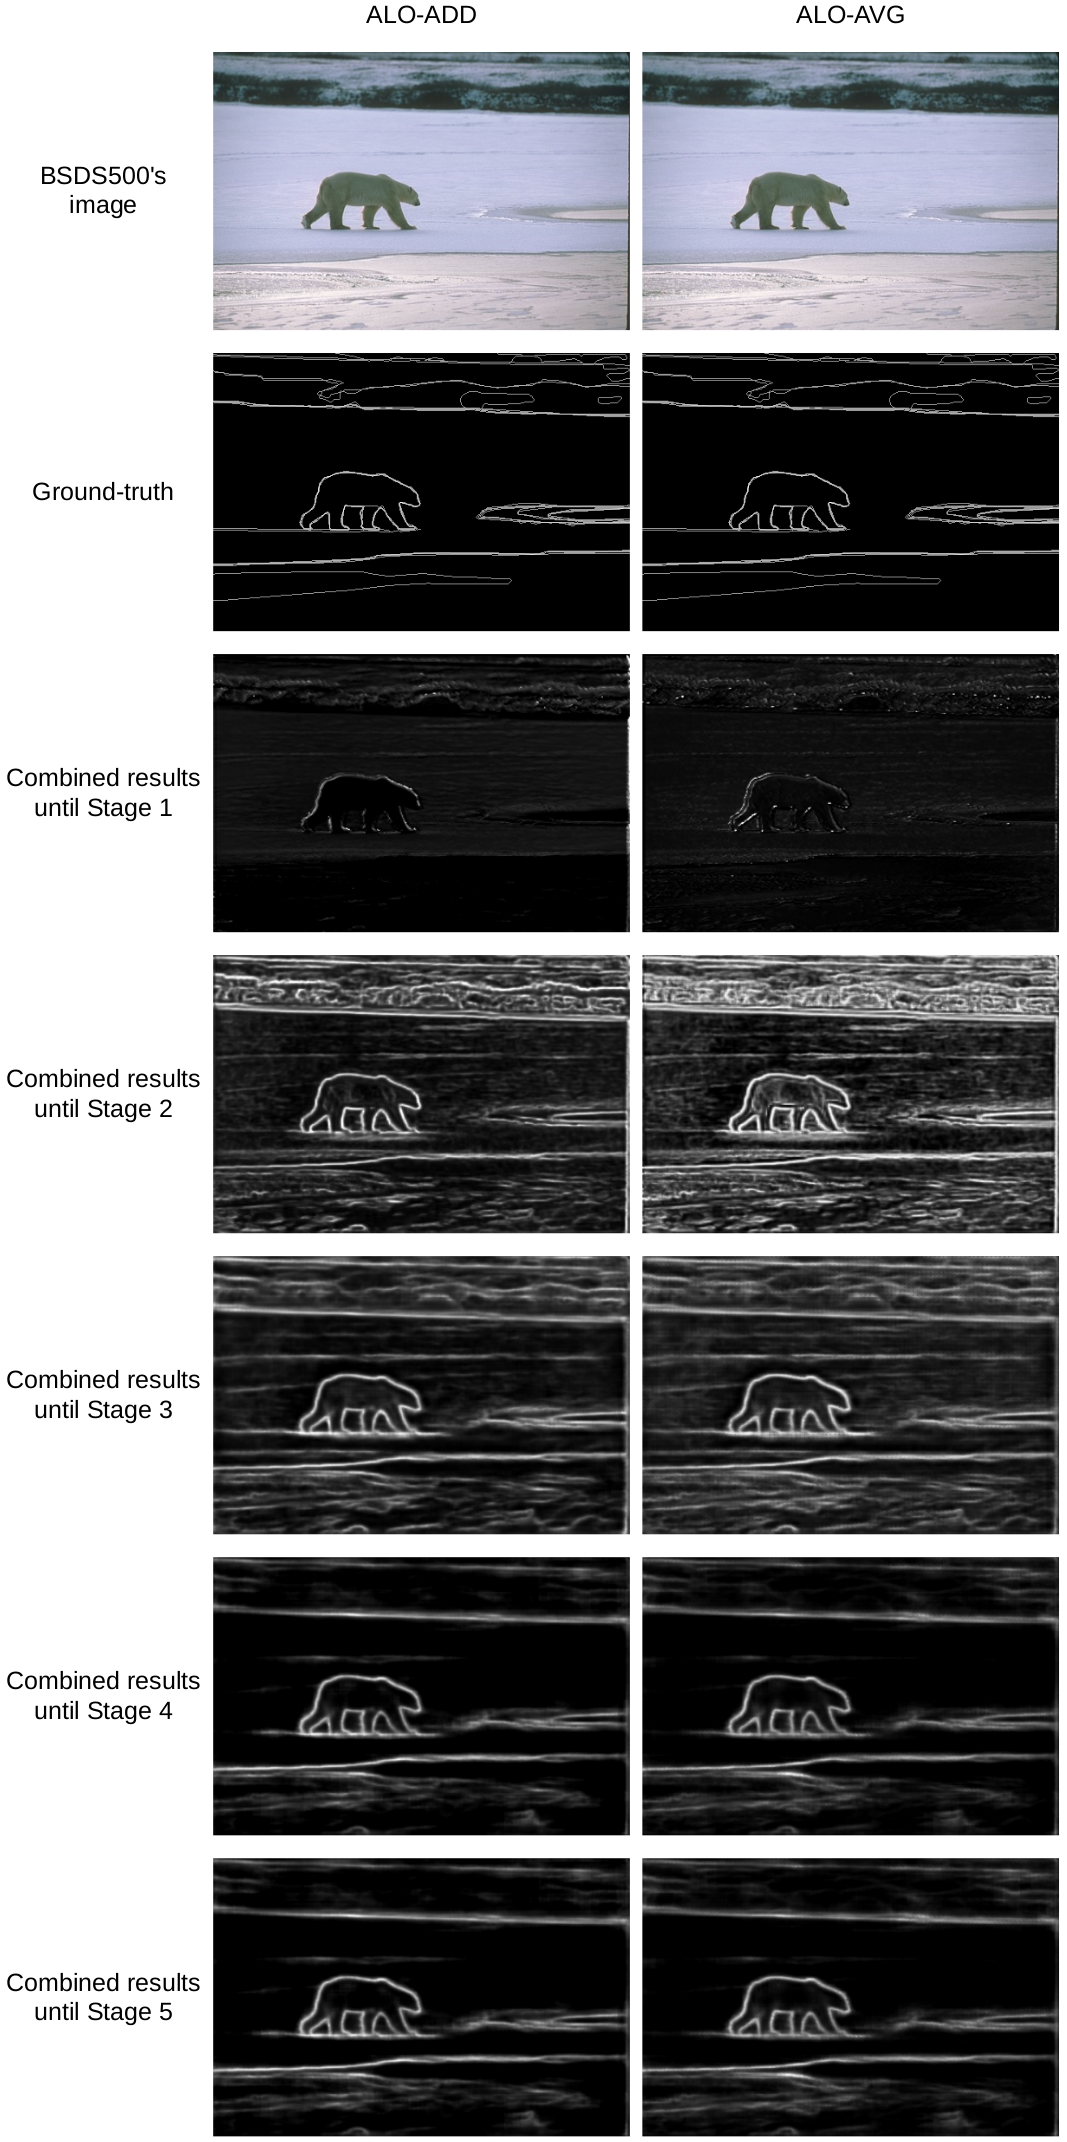
\includegraphics[width=0.9\columnwidth]{../imagens/ilustracoes/cap6_bsds_stage_results.png}
  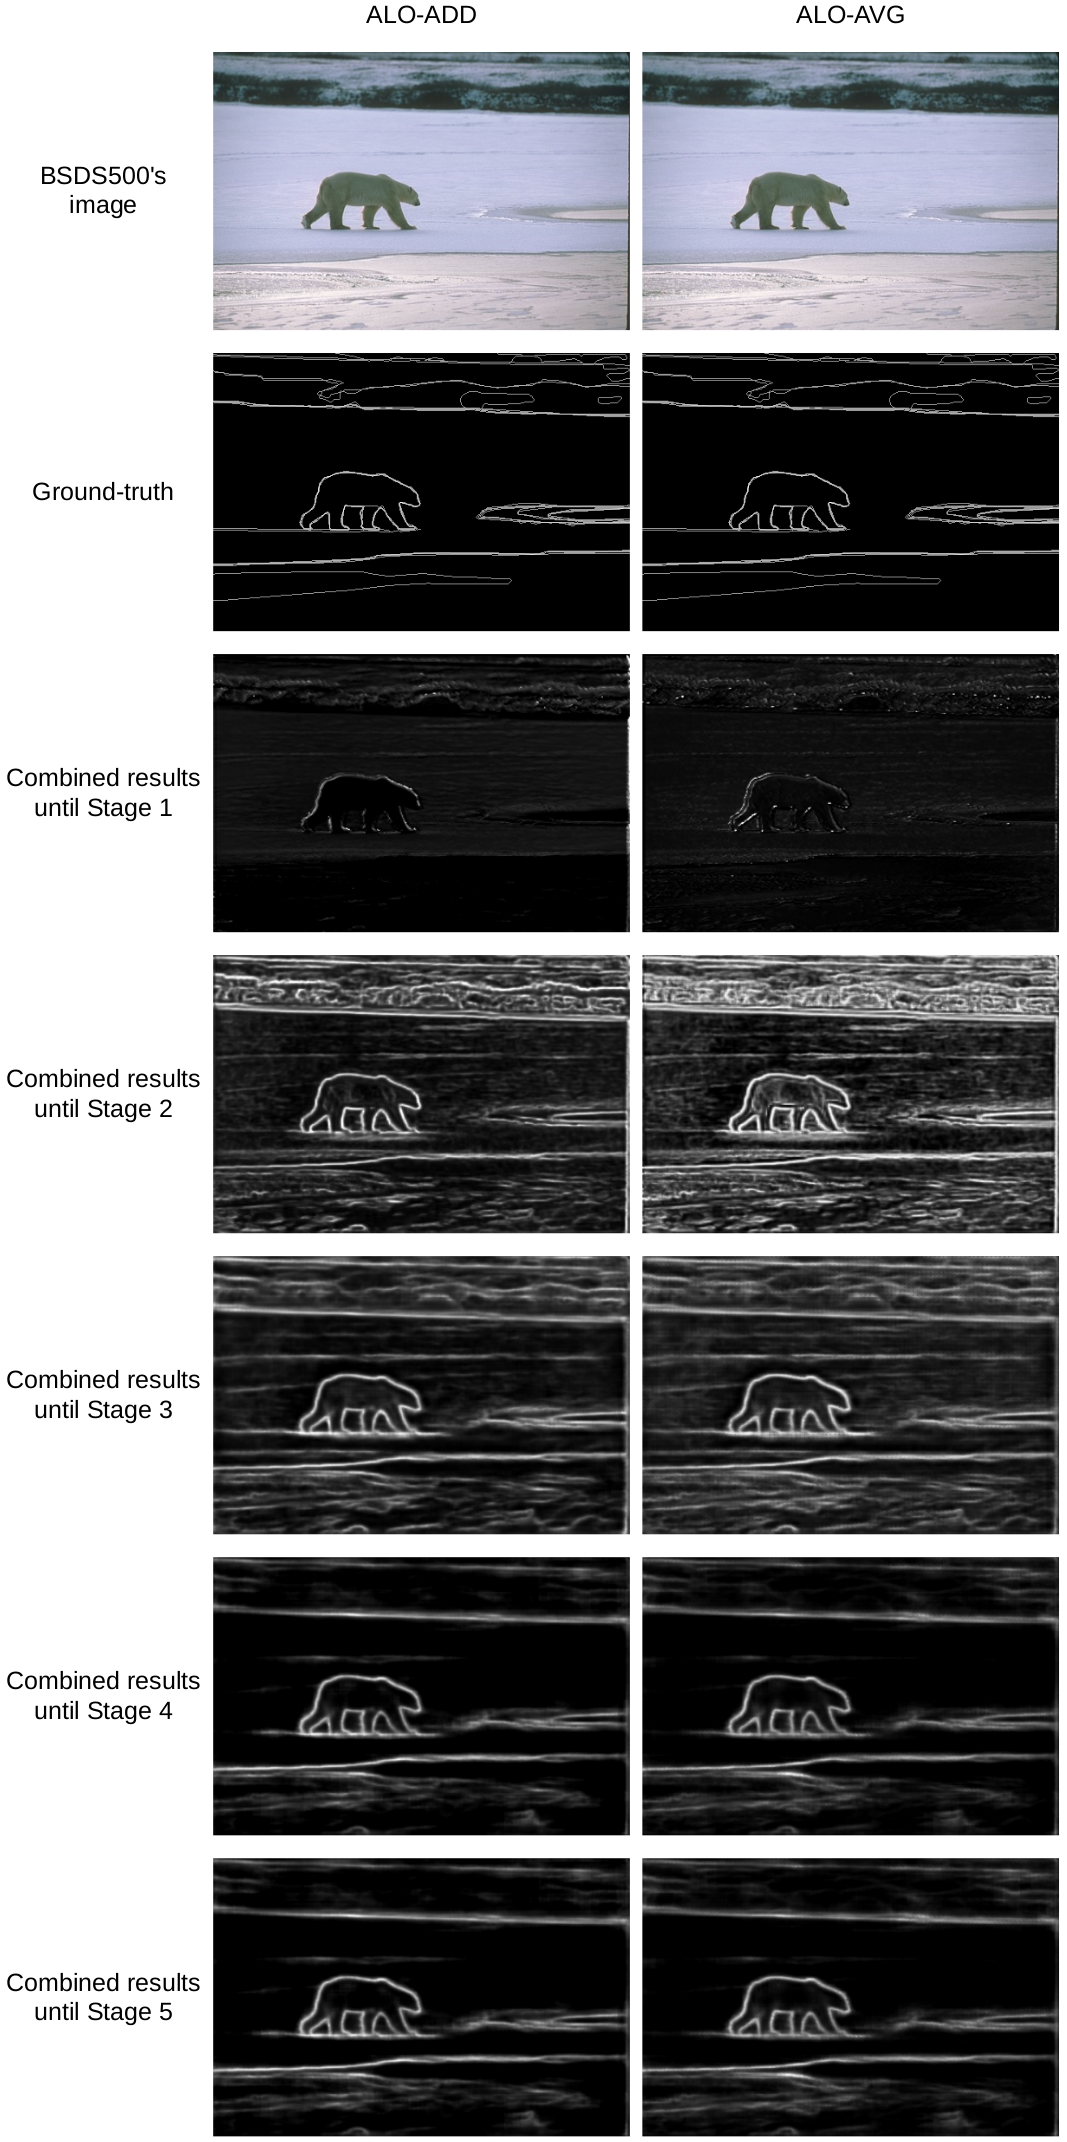
\includegraphics[width=1\columnwidth]{../imagens/ilustracoes/cap6_bsds_stage_results.png} %VISUALIZ
  \caption{Results of ALO-ADD and ALO-AVG methods with side-outputs until each stage, trained with BSDS 500 using MORPH/UPPER ground truth methods.}
  \label{fig:bsds_stage_results}
\end{figure}

% It can be seen in Figure \ref{fig:bsds_stage_outputs} that ALO-ADD and ALO-AVG have different stage output contributions.
% ALO-ADD appears to perform better in stages 1 and 3, while ALO-AVG appears to perform better in stages 2 and 3.
% In the fourth stage, the results shows only blurs, but it is possible to identify some parts only in ALO-AVG, with appears to contribute more with the final output.
% The last stage, as already observed in Figures \ref{fig:bsds_add_side_outputs} and \ref{fig:bsds_avg_side_outputs}, presents only random noises.

Figure \ref{fig:bsds_stage_results} shows a different perspective of stage outputs contribution.
It can be seen that the results become more accurate as more stages are added, except for the last stage, which apparently does not improve the overall performance of the model.

%--------------------------------
\subsection{Experiment 2.3 - Removing last stage layers}
\label{ssec:bsds_subexp3}

After analyzing the intermediate results, as indicated in Section \ref{ssec:bsds_sideout}, a new experiment was developed with the purpose of evaluating the impact of removing layers from the last stage.
As observed in Figures \ref{fig:bsds_stage_outputs} and \ref{fig:bsds_stage_results}, the layers of the fifth stage apparently does not contribute effectively to the final result.

In this experiment, the same parameterization described in Section \ref{ssec:bsds_subexp2} was used, except for the loss decreasing and the minimum learning rate (MinLR).
The value, once fixed into $1 \times 10^{-9}$, was replaced by Equation \ref{eq:min_lr}, where the value depends of the original Learning Rate.
This procedure reduced it to $1 \times 10^{-10}$ in the first phase and $1 \times 10^{-11}$ in last two phases of the protocol.

\begin{equation}
  MinLR = LR \times 10^{-4}
  \label{eq:min_lr}
\end{equation}

Once ALO-AVG and ALO-ADD had similar performance in the previous tests, it was decided to evaluate only one of the methods.
Due to the better performance in the ODS metric, with fewer training epochs, according to Section \ref{ssec:bsds_subexp2}, ALO-AVG was chosen to be used in the following experiments.
Then, ALO-AVG network was completely trained using the protocol defined in Section \ref{ssec:framework_experiments} and the parameterization recently defined.

The 4 and 5-stages ALO-AVG networks had similar values in the first phase of the protocol.
In the second phase, the 4-stage network contains considerably lower losses.
This pattern is also manifest in the last phase, using ALL ground truth.
As results of the lower loss, the 4-stage network produced better results, as described in Table \ref{tab:bsds_subexp3_results}, despite of the bigger number of epochs to reach the best value.

The network training process of the 4-stage ALO-AVG method was carried out in 556 epochs, instead of 409 from regular 5-stages ALO-AVG.
As the network with 4 layers is smaller than the traditional network, each epoch runs faster.
However, even with this advantage, the total training time was about 21.80\% longer than conventional 5-stage ALO-AVG.

% The network training and its comparison with 5-stage ALO-AVG are available in Figures \ref{fig:bsds_4stage_morph} and \ref{fig:bsds_4stage_all}.
% Figure \ref{fig:bsds_4stage_morph} shows similar values for both networks in the first phase of the protocol.
% In the second phase, the 4-stage network contains considerably lower losses.
% This pattern is also manifest in the last phase, using ALL ground truth, as presented in Figure \ref{fig:bsds_4stage_all}.

%Tempo: s4 = 43084+123229+99740=266053 | s5 = 37266+80641+100524=218431

% \begin{figure}%[h!]
%   \centering
%   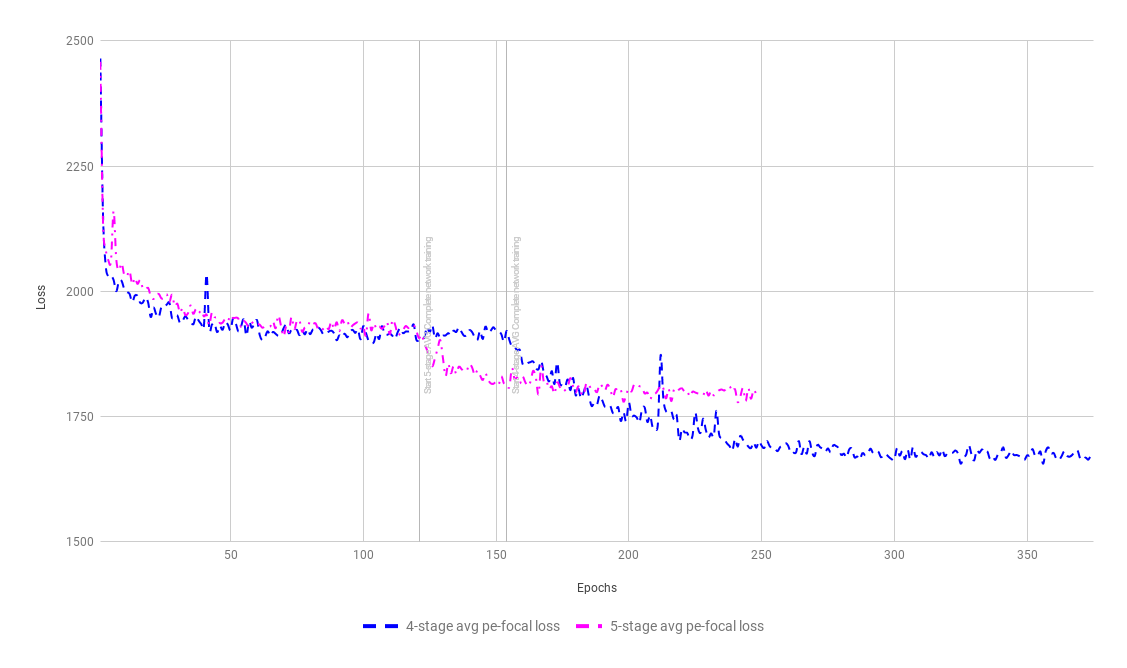
\includegraphics[width=1.\columnwidth]{../imagens/graficos/cap6_bsds_avg_4stage_morph_20200410-0529.png}
%   \caption{Training losses of 4 and 5 stages ALO-AVG versions using MORPH ground truth on BSDS500.}
%   \label{fig:bsds_4stage_morph}
% \end{figure}
% 
% \begin{figure}%[h!]
%   \centering
%   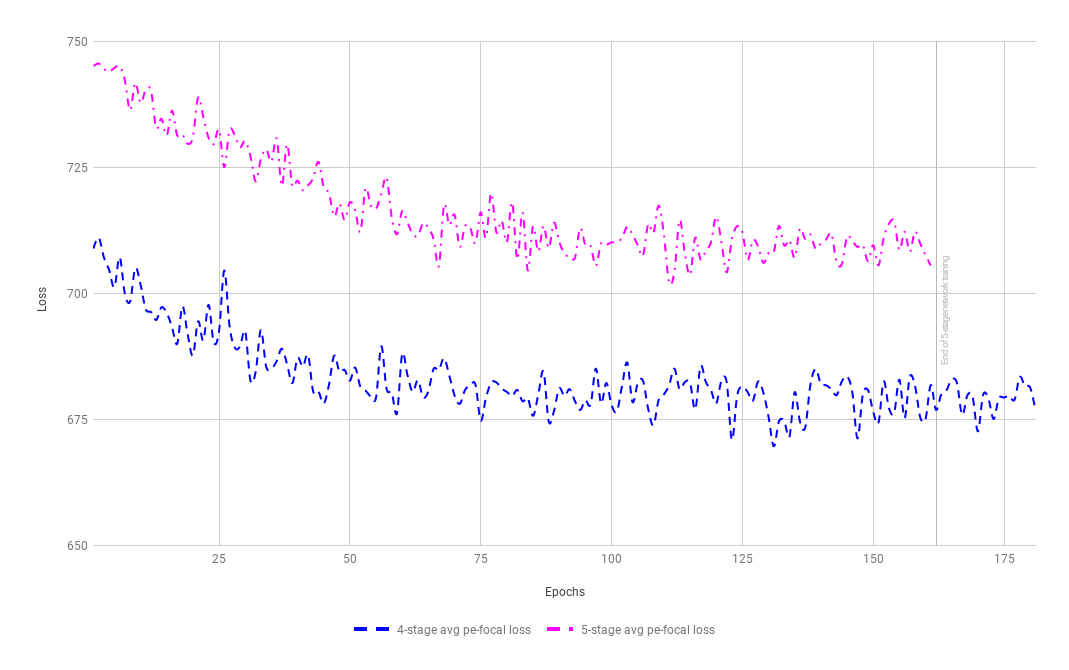
\includegraphics[width=1.\columnwidth]{../imagens/graficos/cap6_bsds_avg_4stage_all_20200410-0529.png}
%   \caption{Training losses of 4 and 5 stages ALO-AVG versions using ALL ground truth on BSDS500.}
%   \label{fig:bsds_4stage_all}
% \end{figure}

% As results of the lower loss, the 4-stage network produced better results, as described in Table \ref{tab:bsds_subexp3_results}, despite of the bigger number of epochs to reach the best value.

\begin{table}%[h!]
  \centering
  \caption{Border detection performance on BSDS500 in Experiment 2.3 (using histogram equalization pre-processing).}
  %\scriptsize
  %\setlength{\tabcolsep}{1em}
  \renewcommand{\arraystretch}{1.5}
  \begin{tabular}{{c}{c}{c}{c}{c}{c}}
    \hline
    Network & Loss & Ground truth & TH & ODS & OIS
    \\
    \hline
    ALO-AVG & PEFL & ALL & 0.17 & 0.7625 & 0.7791
    \\
    \hline
  \end{tabular}
  \label{tab:bsds_subexp3_results}
\end{table}

\subsubsection{Changing data pre processing}
\label{sssec:bsds_pre_process_data}

All previous experiments, including those with the KITTI data set, were done using histogram equalization for each image channel as a pre-processing step.
The technique was chosen due to its possible adaptation to different databases.
However, after all the experiments previously carried out, it was decided to evaluate the subtraction of the means of each channel, using the same parameters described in \cite{VGGNET:2014} paper.

Using VGGNet pre-processing weights, an increase in performance was expected, since the method would equalize the entire database evenly, unlike the previous technique, which adjusted each image separately.
Such a procedure would enable faster and more effective learning.

To assess the change, a naive test was performed using the final weights from the previous experiment.
The network was trained again, only in the last phase of the protocol, using images with the new pre-processing method.
Surprisingly, only this step was able to raise previous results by more than 1\%, to 0.7769 ODS and 0.7913 OIS values.

In order to provide a fair comparison, the network was fully trained using the same parameters described in experiment of Section \ref{ssec:bsds_subexp3}.
The training procedure left 490 epochs and produced the results in Table \ref{tab:bsds_subexp3_results_pre_vgg}.
The results are slightly inferior to training described in the last paragraph, but once it followed the fully protocol, it better represent the behavior of the network.

\begin{table}%[h!]
  \centering
  \caption{Border detection performance on BSDS500 in Experiment 2.3 (using VGG16 pre-processing).}
  %\scriptsize
  %\setlength{\tabcolsep}{1em}
  \renewcommand{\arraystretch}{1.5}
  \begin{tabular}{{c}{c}{c}{c}{c}{c}}
    \hline
    Network & Loss & Ground truth & TH & ODS & OIS
    \\
    \hline
    ALO-AVG & PEFL & ALL & 0.18 & 0.7735 & 0.7876
    \\
    \hline
  \end{tabular}
  \label{tab:bsds_subexp3_results_pre_vgg}
\end{table}

The results provided in this section indicates that the change in the pre-processing method increased the results and reduced the number of training epochs, as expected.
%These results indicates the influence of the data set equalization.
The following experiments, in next sections, will use the same pre-processing method.
  
%--------------------------------
\subsection{Experiment 2.4 - Training Side-Outputs}
\label{ssec:bsds_subexp4}

{\color{red}
The current experiment aims to evaluate if making all side-outputs to produce similar predictions increase overall results.
%This experiment used differents approaches to make network to produce the same result at the side-outputs, to trying to take advantage of multi-scale.
All networks used in this experiment are VGG16 versions with 4 stages and parameterization described in Section \ref{ssec:bsds_subexp3} (including  pre-processing of Section \ref{sssec:bsds_pre_process_data}).
}

\subsubsection{Training each convolution of ALO-AVG with 4 stages}
\label{sssec:train_conv_alo_avg}

The first experiment aimed to evaluate the possible improvement in the results of the ALO-AVG network by training it with loss functions after each convolutional layer.
The network was trained with 11 loss functions, one for each convolution and one for the final output, with merged output.

%This training variation sought to evaluate the gains in the production of multi-scale outputs with the network that obtained the best results in the previous experiments.
%However, despite the good results in the previous experiments, the network had difficulties to learn, possibly due to the excess of outputs and loss functions.

After training, it was observed that the network had more difficulty to learn when compared to previous architectures, resulting in a worse performance. \ref{tab:bsds_subexp4_results}.
As result, the network reached an ODS value of 0.7259 and an OIS value of 0.7418 after 271 training epochs.

It was observed, in the individual evaluation of the outputs, that some intermediate results, mainly in the first stages, did not present useful information (map without any border) and that several others, specially at the end, presented many noises, generating many false positives and inaccurate edges.

%Excessive side-outputs may have caused difficulties in knowledge propagation between layers of the network.
%Also, the network trained only for 271 epochs, whats indicates that the network was unable to learn properly.
%The color and border adjustments, as shown in Figure \ref{fig:bsds_avg_side_outputs}, were compromised, since the layer alone sought to generate an output close to the border map.

%As result, the network reached an ODS value of 0.7259 and an OIS value of 0.7418 after 271 training epochs.
%Evaluating the results presented in Table \ref{tab:bsds_subexp4_results}, it is possible to see that the network had considerably lower results than other networks described in Section \ref{sssec:bsds_pre_process_data}.

%The low number of training epochs, added to the low results obtained, indicates that the network was unable to learn properly and that the high number of side-outputs hindered learning.

\subsubsection{Training each stage of SLO-AVG with 4 stages}
\label{sssec:train_stage_slo_avg}

Due to the poor results in the last experiment, it was proposed to reduce the number of side-outputs that should be trained.
Following the context of this work and the previously used networks, it was decided to use the SLO-AVG net.
The network was trained with 5 loss functions, one for each stage and one for the final average output.

Since early epochs, this version of the network produced smaller training and validation loss values than the previous ALO-AVG experiment.
After 476 training epochs, the network produced 0.7640 ODS and 0.7795 OIS values, which is almost 6\% better than the previous network.
Nonetheless, these results are smaller than the results of ALO-AVG without multiple loss functions.

\subsubsection{Training a fine and a coarse output}
\label{sssec:train_alo_plus}

Inspired in Convolutional Oriented Boundaries network \cite{COB:2016}, this new experiment aimed to evaluate the creation of a fine and a coarse output.
To produce it, a new version of ALO-AVG network was created and named ALO-PLUS.

The network contained two side-outputs, a fine one, containing the average of the initial intermediate outputs (convolutions in stages 1 to 3) and a coarse one, containing the average of the outputs of the fourth stage.
The outputs were trained independently.
To produce a single result, a late merging method was created, with the average of both results.

The BSDS500 evaluation of the results produced by this ALO-PLUS network resulted in 0.7573 ODS and 0.7729 OIS values (the training procedure left 534 epochs).
The results can be considered intermediate when compared to values of other experiments carried out in this work.

%It is also important to indicate that this experiment, with a delayed fusion method, allows the choice of a more appropriate technique to combine the network outputs after training.
%espite this, only a visual assessment of the use of weights in each output was made, but no improvement was noticed. 
%Then, it was not evaluated using the BSDS500 benchmark.

\subsubsection{Training each stage of SLO-ADD  with 4 stages}
\label{sssec:train_stage_slo_add}

Due to the good results of the SLO-AVG in the experiment described in Section \ref{sssec:train_stage_slo_avg} and the similar results reached using ADD and AVG operations in experiments in Sections \ref{ssec:bsds_subexp2} and \ref{ssec:bsds_subexp2}, a new experiment was carried out using SLO-ADD network.
The network was trained with 5 loss functions, one for each stage and one for the final output.

The training of SLO-ADD was slower to other networks, with exactly 700 epochs.
Despite the longer training time, SLO-ADD produced poorly 0.7117 ODS and 0.7231 OIS values, what is considerably worse than SLO-AVG and other networks.

The results visually indicated the edges, however, presented numerous noises, which could be considered as soft edges.
However, it was noticed that the hue of the soft edges was very similar to the hard edges, which probably caused the poorly results.
This small difference could lead to multiple false positives, even with different thresholds.

\subsubsection{Side-outputs training summary}
\label{sssec:sideout_train_summary}

{\color{red}
The summary of the experiments performed in this section are presented in Table \ref{tab:bsds_subexp4_results}.
Analyzing the results, it is possible to see that SLO-AVG network had the best ODS and OIS values.
However, the results are smaller than those achieved by ALO-AVG net in Section \ref{sssec:bsds_pre_process_data}.
}

% \begin{table*}%[h!]
%   \centering
%   \caption{Border detection performance on BSDS500 for SLO and ALO networks with side-output training.}
%   \scriptsize
%   %\setlength{\tabcolsep}{1em}
%   \renewcommand{\arraystretch}{1.5}
%   \begin{tabular}{{c}{c}{c}{c}{c}{c}{c}}
%     \hline
%     Network & Loss & Trained side-outputs & Ground truth & TH & ODS & OIS
%     \\
%     \hline
%     ALO-AVG & PEFL & 11 & ALL & 0.18 & 0.7259 & 0.7418
%     \\
%     SLO-AVG & PEFL & 5 & ALL & 0.18 & 0.7640 & 0.7795
%     \\
%     ALO-PLUS & PEFL & 2 (fine and coarse) & ALL & 0.18 & 0.7573 & 0.7729
%     \\
%     SLO-ADD & PEFL & 5 & ALL & 0.18 & 0.7117 & 0.7231
%     \\
%     \hline
%   \end{tabular}
%   \vspace{0.2cm}
%   \label{tab:bsds_subexp4_results}
% \end{table*}

\begin{table}%[h!]
  \centering
  \caption{Border detection performance on BSDS500 in Experiment 2.4.}
  %\scriptsize
  %\setlength{\tabcolsep}{1em}
  \renewcommand{\arraystretch}{1.5}
  \begin{tabular}{{c}{c}{c}{c}{c}{c}{c}}
    \hline
    Network & Loss & Side-out. & GT & TH & ODS & OIS
    \\
    \hline
    ALO-AVG & PEFL & 11 & ALL & 0.18 & 0.7259 & 0.7418
    \\
    SLO-AVG & PEFL & 5 & ALL & 0.18 & 0.7640 & 0.7795
    \\
    ALO-PLUS & PEFL & 2 & ALL & 0.18 & 0.7573 & 0.7729
    \\
    SLO-ADD & PEFL & 5 & ALL & 0.18 & 0.7117 & 0.7231
    \\
    \hline
  \end{tabular}
  \vspace{0.2cm}
  \label{tab:bsds_subexp4_results}
\end{table}


%--------------------------------
\subsection{Experiment 2.5 - Improving ALO network}
\label{ssec:bsds_subexp5}

% After analyse the experiments in Section \ref{ssec:bsds_subexp3}, and inspired in some recent papers that create auxiliary branches in their network, as \cite{Cumulative:Song20181847}, \cite{LearningHybrid:Hu2018377} and \cite{He:2019}, a new experiment was proposed.
% To create an auxiliary branch, the first step was adding some new convolutional layers in each side-output of the 4-stage ALO network.
% 
% The network was trained with this new architecture for a few epochs and, before evaluate the results, it was observed that the loss increased and the network also left more training epochs to converge properly.
% After review the side-output block, it was decided to counter the recent trend of auxiliary branches and remove each possible extra layer of that block.

As described in Section \ref{cap5_saidas_laterais}, ALO's side-output blocks are composed by an $1 \times 1$ convolution, followed by a transposed convolution.
It was observed that the $1 \times 1$ convolution could be removed without great impact in the network, except for the possibility of making it a little less stable.

Due to the architectural change and in order to differentiate it from the ALO networks, the new neural network was named \textit{eXtreme All-layers Outputs}  (XLO).
% The network was created only with AVG and ADD operations, due the poor performance of MAX in previous tests, as described in Sections \ref{ssec:bsds_subexp1} and \ref{ssec:basic_pred_eval}.
% The XLO network was trained using the default protocol with AVG and ADD merging methods, ALL and UPPER ground truths and the following parameterization, similar to that described in Section \ref{sssec:bsds_pre_process_data}, and summarized below.
The XLO network was trained using the default protocol with AVG and ADD merging methods, ALL and UPPER ground truths and the following parameterization different from the default one, described in Section \ref{ssec:framework_experiments}.

\begin{itemize}
  \item Learning rate: $1 \times 10^{-6}$ (first step) and $1 \times 10^{-7}$ (others)
  \item Learn. decay: $1 \times 10^{-10}$ (first step) and $1 \times 10^{-11}$ (others)
  \item Loss: PEFL ($\gamma$=1.0; $\alpha$=0.25)
  \item Pre-processing: VGG-16
\end{itemize}

% \begin{itemize}
%   \item Learning method: SGD
%   \item Activation: ReLU
%   \item Learning rate: $1 \times 10^{-6}$ (first step) and $1 \times 10^{-7}$ (others steps)
%   \item Learning decay: $1 \times 10^{-10}$ (first step) and $1 \times 10^{-11}$ (others steps)
%   \item Batch size: 8 images
%   \item Loss: PEFL ($\gamma$=1.0; $\alpha$=0.25)
%   \item Initial weights: VGG-16
%   \item Pre-processing: VGG-16
%   \item Training samples: 9690 images 
%   \item Validation samples: 1710 images
%   \item Image size: $384 \times 288$
% \end{itemize}

After training the networks, the results were evaluated and summarized in Table \ref{tab:bsds_subexp5_results}.
The number of training epochs is available in Table \ref{tab:bsds_subexp5_epochs} and the some visual samples of the best results are available in Figure \ref{fig:cap6_expr5_bsds_visual}.
It is possible to see in Table \ref{tab:bsds_subexp5_results} that the results increased when compared to Section \ref{ssec:bsds_subexp3}, the best results so far.
Also, the number of training epochs has not increased considerably when compared to previous experiments.

\begin{table}%[h!]
  \centering
  \caption{Border detection performance on BSDS500 for XLO-ADD and XLO-AVG in Experiment 2.5.}
  %\scriptsize
  %\setlength{\tabcolsep}{1em}
  \renewcommand{\arraystretch}{1.5}
  \begin{tabular}{{c}{c}{c}{c}{c}{c}{c}}
    \hline
    Network & Loss & G. truth & TH & ODS & OIS & AP
    \\
    \hline
    XLO-ADD & PEFL & ALL & 0.18 & 0.7760 & 0.7901 & 0.7023
    \\
    XLO-ADD & PEFL & UPPER & 0.30 & 0.7741 & 0.7897 & 0.6846
    \\
    \hline
    XLO-AVG & PEFL & ALL & 0.19 & \textbf{0.7796} & 0.7937 & \textbf{0.7209}
    \\
    XLO-AVG & PEFL & UPPER & 0.31 & 0.7793 & \textbf{0.7961} & 0.6966
    \\
    \hline
  \end{tabular}
  \label{tab:bsds_subexp5_results}
\end{table}

\begin{table}%[h!]
  \centering
  \caption{Number of training epochs in Experiment 2.5.}
  %\scriptsize
  %\setlength{\tabcolsep}{1em}
  \renewcommand{\arraystretch}{1.5}
  \begin{tabular}{{c}{c}{c}{c}{c}{c}{c}}
    \hline
    Ground truth & XLO-ADD & XLO-AVG 
    \\
    \hline
    MORPH / ALL & 527 & 442
    \\
    MORPH / UPPER & 534 & 596
    \\
    \hline
  \end{tabular}
  \label{tab:bsds_subexp5_epochs} 
\end{table}

The results indicating a better behavior of XLO networks when compared to all previous versions of ALO networks, although the performance is not considerably superior.
However, due to the performance gain in all versions of the network, the XLO network can be considered superior to the ALO network and, consequently, to the SLO network.

To compare the speed of the best versions of XLO and ALO networks, it was created the Table \ref{tab:bsds_fps}.
This table contains the speed performance of both networks to predict images\footnote{~The images that fed the network had the size of $384 \times 288$ and were resized to the default image size of $321 \times 481$ inside the FPS evaluation.}. %\footnote{~Using XLO's $384 \times 288$ weights to fed a $320 \times 480$ network and without any image resizing, the network produced 0.7768 ODS and 0.7920 OIS values at 54.4 FPS.}.
As can be seen in Table \ref{tab:bsds_fps}, XLO network is 8,74\% faster than ALO network, with better ODS and OIS values.

\begin{table}%[h!]
  \centering
  \caption{FPS performance evaluation of ALO-AVG with 4 stages and XLO-AVG network.}
  %\scriptsize
  %\setlength{\tabcolsep}{1em}
  \renewcommand{\arraystretch}{1.5}
  \begin{tabular}{{c}{c}{c}}
    \hline
    GPU & ALO-AVG & XLO-AVG
    \\
    \hline
    %Nvidia GTX 1080 & 41.2 & \textbf{44.8} (288x384)
    Nvidia GTX 1080 & 41.2 & \textbf{\myFPS}
    %\\
    %Nvidia GTX 1080 & 58.0 & \textbf{54.4} (320x480)
    \\
    \hline
  \end{tabular}
  \label{tab:bsds_fps} 
\end{table}

% \begin{figure*}
%   \centering
%   \caption{Predictions of the XLO-AVG, with ALL ground truth and it best threshold.}
%   \captionsetup[subfigure]{labelformat=empty}
%   \subfloat[BSDS500 image\label{fig:cap6_expr5_img}]{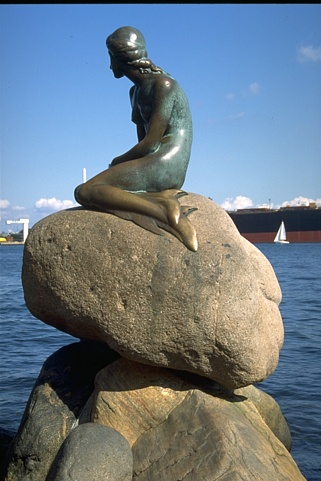
\includegraphics[width=0.24\textwidth]{../imagens/ilustracoes/cap6_bsds_372019.jpg}}
%   \hfill
%   \subfloat[Ground truth\label{fig:cap6_expr5_gt}]{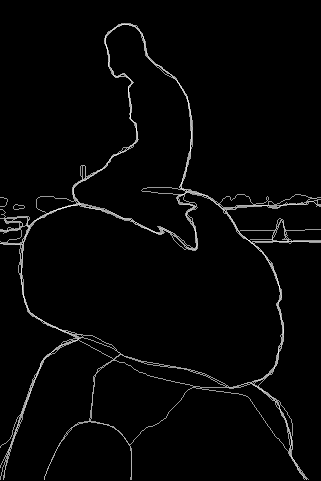
\includegraphics[width=0.24\textwidth]{../imagens/html/372019_upper.png}}
%   \hfill
%   \subfloat[XLO-AVG\label{fig:cap6_expr5_avg}]{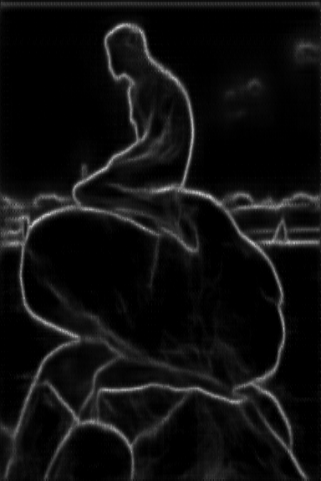
\includegraphics[width=0.24\textwidth]{../imagens/ilustracoes/cap6_bsds_372019_xlo_avg_all_20200701.png}}
%   \hfill
%   \subfloat[XLO-AVG (0.19)\label{fig:cap6_expr5_avg_th}]{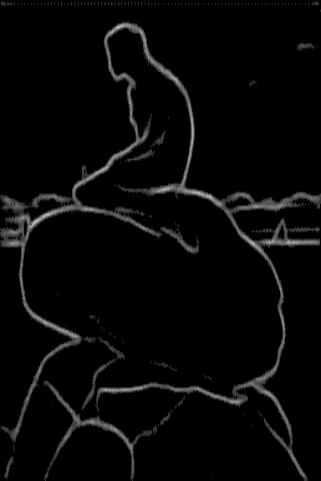
\includegraphics[width=0.24\textwidth]{../imagens/ilustracoes/cap6_bsds_372019_xlo_avg_all_20200701_019.png}}
%   \hfill
%   \label{fig:cap6_expr5_bsds_visual}
% \end{figure*}

% \begin{figure*}%[h!]
%   \centering
%   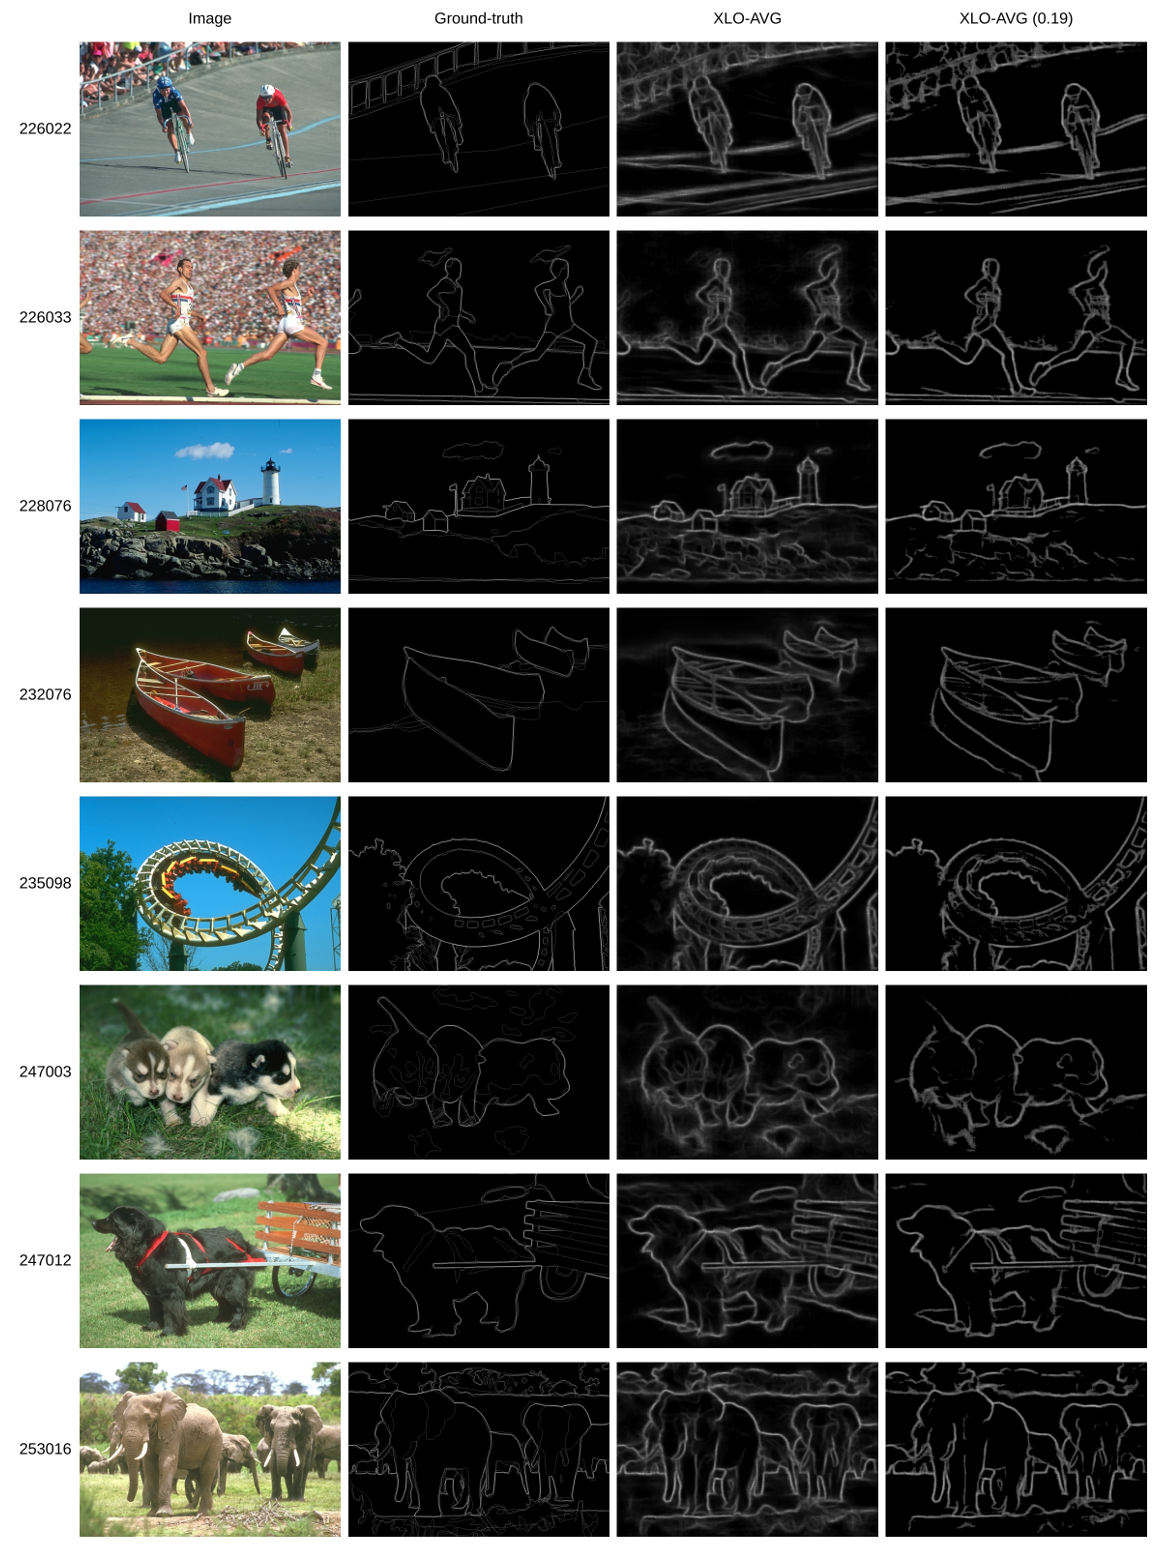
\includegraphics[width=0.7\textwidth]{../imagens/apendice/appendix-horiz-09.png}
%   \caption{Results of XLO-AVG method trained with BSDS 500 using MORPH/ALL ground truth methods.}
%   \label{fig:cap6_expr5_bsds_visual}
% \end{figure*}

\begin{figure*}%[h!]
  \centering
  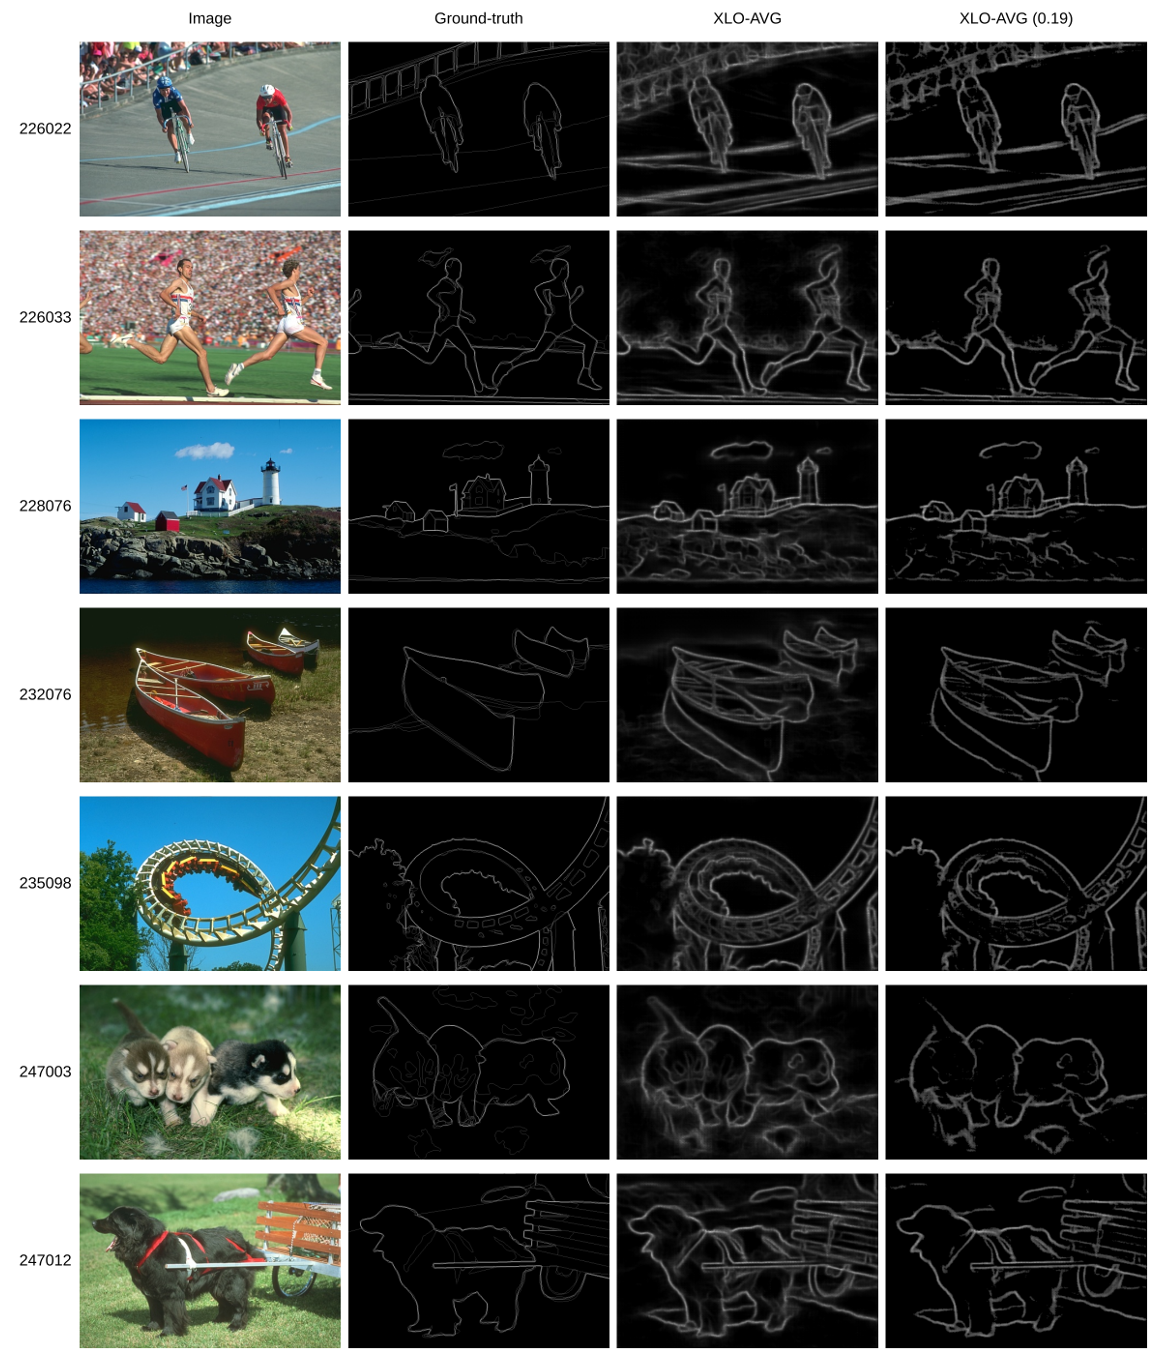
\includegraphics[width=0.9\textwidth]{../imagens/apendice/appendix-horiz-09_v2.png}
  \caption{Results of XLO-AVG method trained with BSDS 500 using MORPH/ALL ground truth methods.}
  \label{fig:cap6_expr5_bsds_visual}
\end{figure*}


%--------------------------------
\begin{comment}
\subsection{Experiment Summary}
\label{ssec:bsds_summary}

{\color{blue}
The evolution of results due to experiments using BSDS500 are available in Figure \ref{fig:bsds_experiments_evolution}.
The figure summarizes the experiments in the BSDS500 dataset, indicating the main modifications at each step.
The figure was created to facilitate the understanding of each of the experiments, indicating the main modifications carried out.
}

\begin{figure*}%[h!]
  \centering
  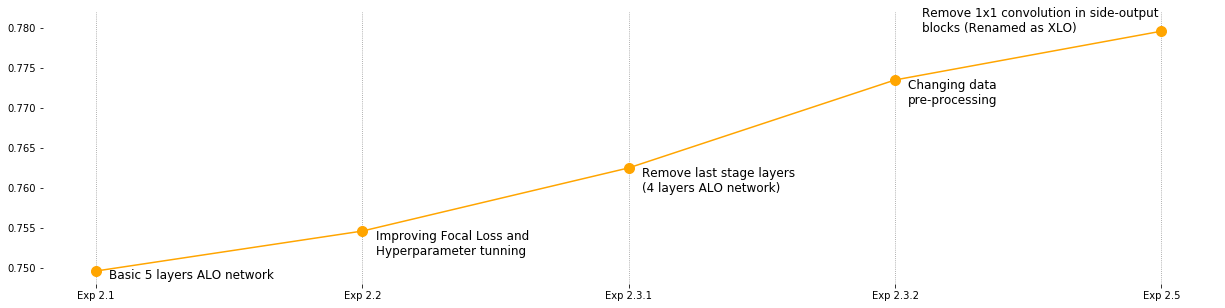
\includegraphics[width=0.9\textwidth]{../imagens/visualiz_dados/bsds_results_evolution.png}
  \caption{Results of ALO-AVG due experiments.}
  \label{fig:bsds_experiments_evolution}
\end{figure*}
\end{comment}
